\chapter{Vida Decision Support System for COVID-19 Response} \label{ch:vida}


\section{Chapter Purpose \& Structure} \label{sec:vida-purpose}

This chapter details an application of the \acf{evdt} Framework for supporting \acf{covid} response in several different regions around the world, varying in size from municipalities to multiple provinces. It thus serves as a case study intended both to demonstrate the utility of the framework and to be a useful reference for those seeking to apply the framework themselves. In this way, this chapter seeks to address Research Question 2: "Does the \ac{evdt} Framework effectively support decision-making in in complex \acf{sets}?" It accomplishes this by providing a case study demonstration of Research Deliverables 2a, 2b, and 2c: 

\begin{enumerate}[label=\emph{\alph*},itemsep=0pt,parsep=0pt]
	\item{System architecture analyses of each of the case studies} 
	\item{Development of an \ac{evdt}-based \acf{dss} for each of the case studies} 
	\item{An interview-based assessment of the development process and usefulness of each \ac{dss}} 
\end{enumerate}

It should be noted that this case study differs from that presented in Chapter \ref{ch:mangroves} in several key ways and in many ways is quite unlike the originally envisioned \ac{evdt} use case detailed in Chapter \ref{ch:evdt}. Rather than dealing with a particular, relatively small study area, this case study includes several distinct study areas of varying sizes (some quite large) with similar but not identical problems to be addressed (the impacts of \ac{covid} manifested quite differently around the world). While there were certainly gaps in our understanding of mangrove health and ecosystem services, these gaps paled in comparison to our understanding of \ac{covid} dynamics and impacts, particularly early in the pandemic (when this project was taking place). 

Finally, due to the urgency and complexity of the \ac{covid} pandemic, a much more iterative \ac{evdt} Framework process was used, with individual steps abbreviated. For instance, during the initial \acf{saf}, we did not contact and formally interview all identified stakeholders, as this would have been quite time consumptive both in terms of the number of such stakeholders across the study areas and their availability for an interview in the early days of the pandemic. Instead, we relied upon multiple iterative cycles to incorporate the perspectives and needs of additional stakeholders over time. Figure \ref{fig:saf-comparison} shows this in a graphical form.

\begin{figure}[!htb]
	\centering
	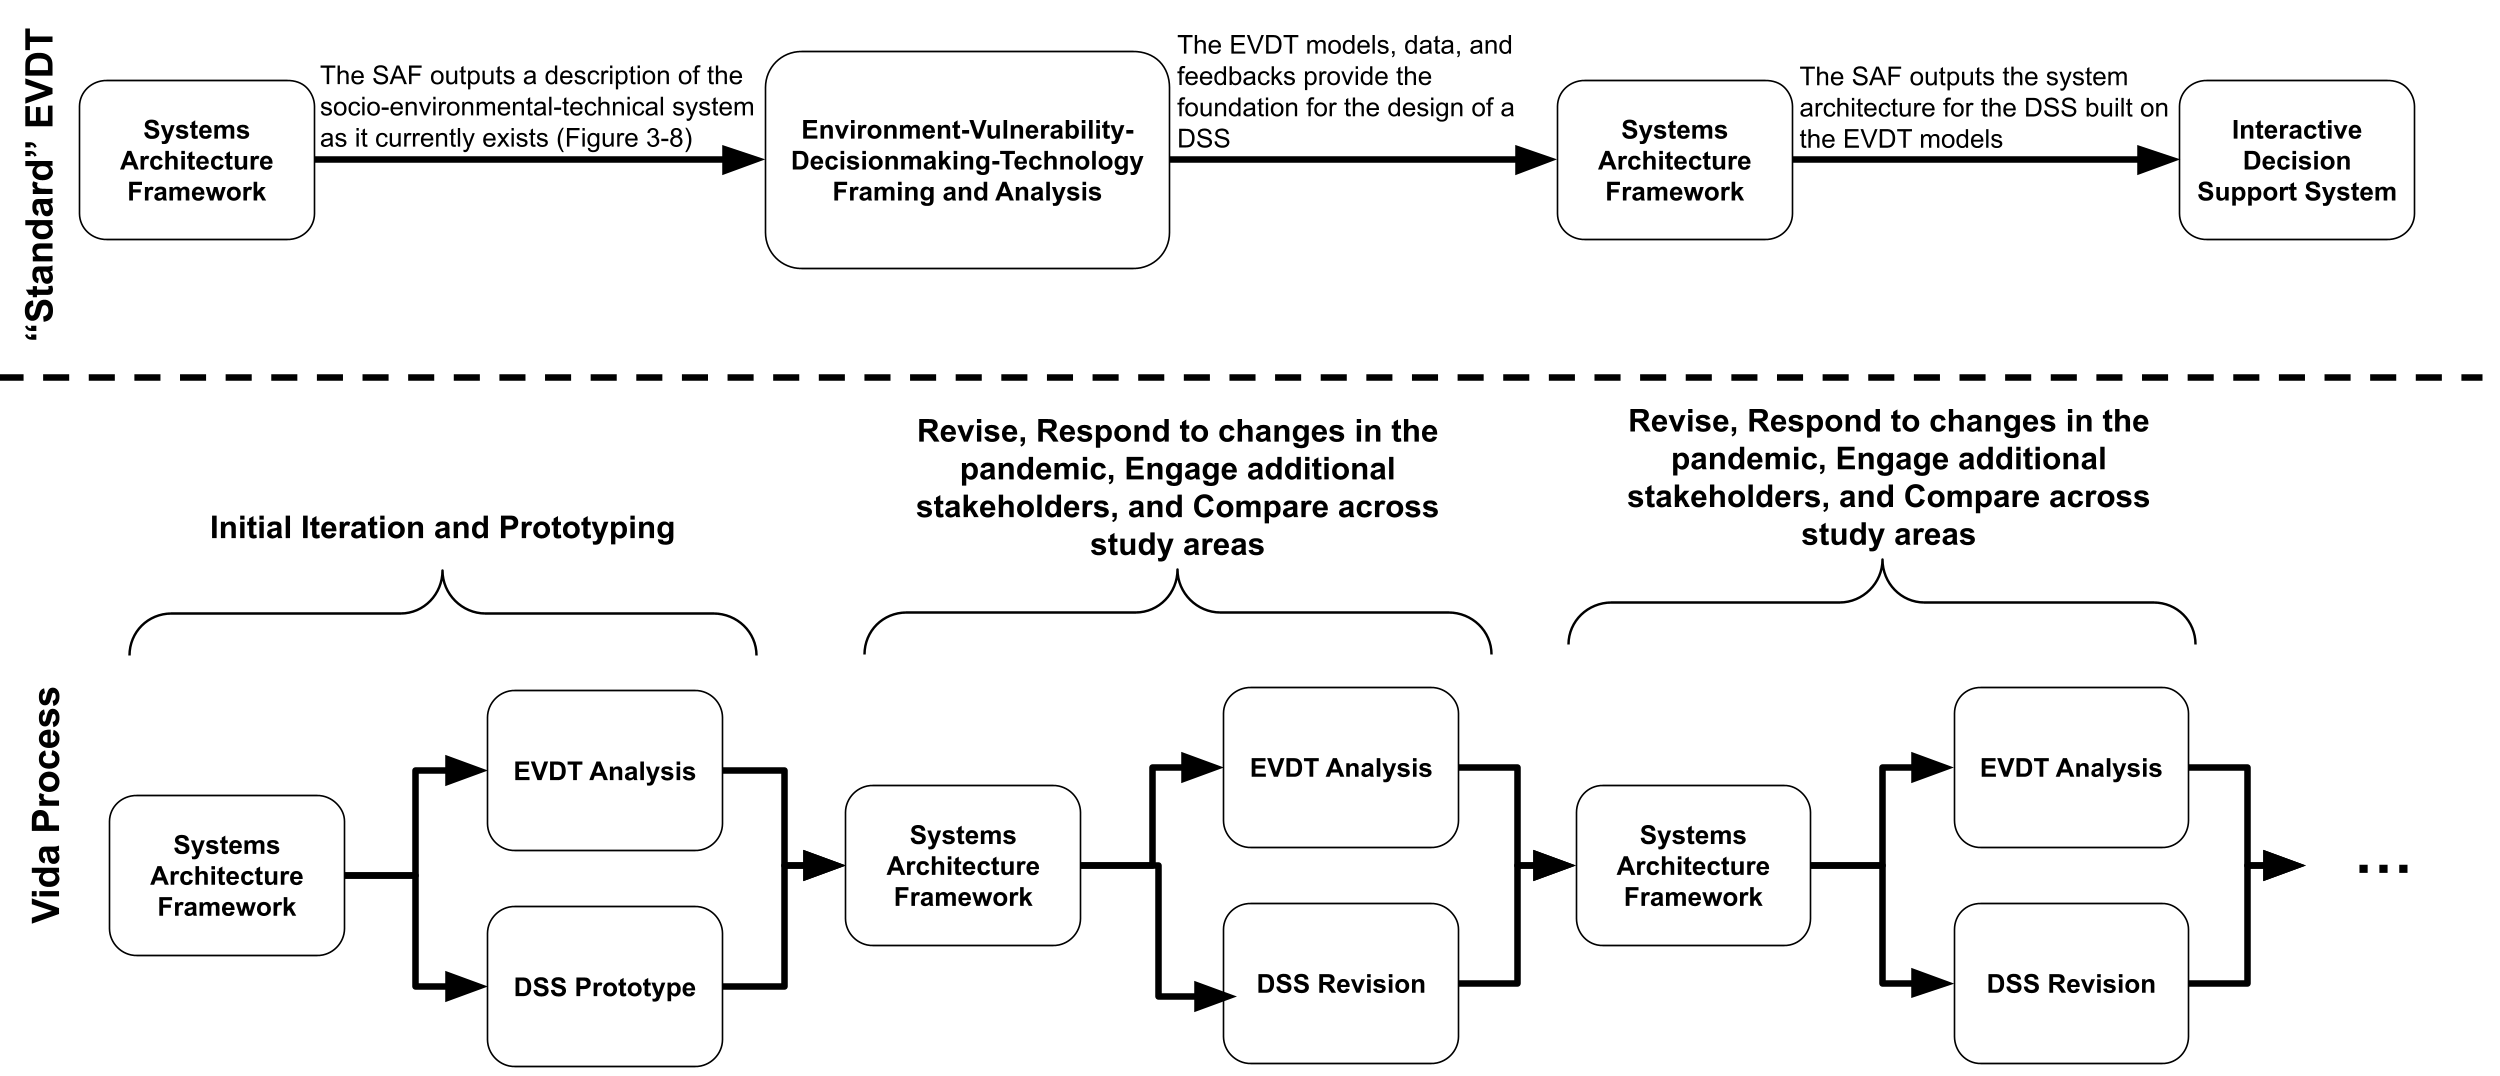
\includegraphics[width=0.9\textwidth]{Figures/chap5/saf-comparison.png}
	\caption[Comparison of the standard EVDT Framework with the Vida Process]{Comparison of the standard EVDT Framework (top, showing only the middle steps) with the process used during the Vida project (bottom)}
	\label{fig:saf-comparison}
\end{figure}


These factors raise the question of why this case study is included in this thesis at all. I include it for three primary reasons. First, this was the first of the ``second generation" \ac{evdt} projects and thus represented our first chance to re-use assets from earlier projects and make use of lessons learned. Second, partially due to these notable differences, this case study resulted in important lessons for the \ac{evdt} Framework that were key to its current formulation. Finally, I think it important to show how the framework does (and does not) perform under the stresses of urgency and complexity.
	
Despite these differences in process, the structure of this chapter will still follow the components of the standard framework laid out in Section \ref{sec:framework}. Each section will present a summary of the overall methods employed and results obtained, rather than detailing each of the iterations of Figure \ref{fig:saf-comparison}. Similarly, this chapter focuses on an overview of the Vida project across study areas, employing some highlights and examples from specific study areas as needed, but not comprehensively covering each.

It starts by walking through the steps of the \acf{saf} as applied to this case study in Section \ref{sec:vida-saf}. These are separated into the methodology used for each step of the \ac{saf} (Section \ref{sec:vida-saf-method}) and the results of each step (Section \ref{sec:vida-saf-result}. Here I outline the various study areas; explain the nature of stakeholder interactions for the project; show how stakeholder needs align and vary across the study areas; and synthesize particular topics of interest for analysis and inclusion in the \ac{dss}.

Then, in Section \ref{sec:vida-evdt}, it shall turn to showing relevant datasets and analysis as applied through the \acf{evdt} models. These are also separated into methodology (Section \ref{sec:vida-evdt-method}) and results (Section \ref{sec:vida-evdt-result}. Unlike Chapter \ref{ch:mangroves}, there is no primary flow to these analyses (something that is discussed towards the end of this chapter). Environmental analyses included tracking (in-situ) air quality and urban nightlights. Public health relied predominantly on a systems dynamics model of cases over time. Vulnerability considered various forms of economic and human impacts, such as telecommunications-based mobility trends and ship traffic. Decision-making focused on government policies to reduce the spread of \ac{covid} such as mask mandates and public area closures.

These are then integrated into a prototype \ac{dss} in Section \ref{sec:vida-dss} that built upon the code base from the previous chapter's \ac{dss}, displaying spatiotemporal data and generating public health scenarios based on user inputs. This \ac{dss} could be set to each of the study areas and had customized historical data and simulation parameters for each.

Section \ref{sec:vida-collab} lays out how various stakeholders were collaborated with beyond the setting of requirements during the \ac{saf} process. This was a key point of this case study as the fact that this project covered multiple stakeholders meant that in some ways, this project consisted of multiple, parallel \ac{evdt} projects. It thus had new opportunities for collaboration across study areas.

Section \ref{sec:vida-discuss} provides the primary discussion of the chapter, considering the various methodological limitations at each stage of this project and what lessons were learned for the \ac{evdt} Framework as a whole; in particular the benefits of multi-study-area or multi-project communication and collaboration, and the importance of clearly scoped problem and use. These lessons are revisited in Chapter \ref{ch:conclusion} as part of a broader evaluation of the \ac{evdt} Framework.

It should be noted that, as stated in Section \ref{sec:questions}, each case study also has its own objectives beyond supporting a chapter of this thesis. In this case, that means supporting \ac{covid} pandemic response in each of the participating metropolitan areas. Readers interested in environmental analyses performed in the course of this research are pointed to Sections \ref{sec:vida-evdt-e-method}, \ref{sec:vida-evdt-e-result}, and \ref{sec:vida-discuss}.

\section{Case Study Acknowledgments}

The \ac{evdt} Framework calls for collaboration. I thus think it only fitting that I briefly acknowledge certain key participants in the Vida project. All \ac{evdt} projects, by their nature, involved a large number of participants. That said, in Chapter \ref{ch:mangroves}, the primary Space Enabled participant was myself and, while Technical Area Experts provided advice and actionable information, I conducted the direct implementation of the analyses and the \ac{dss}. This is not the case in the Vida case study. Various other individuals provided analysis and coding labor throughout the process. I will do my best to refer to them by name throughout the chapter, but here is a brief summary of direct contributions:

\begin{itemize}[itemsep=0pt,parsep=0pt]
	\item{Seamus Lombardo: Served as the point-of-contact for the Indonesia and (sometimes) the Angola collaborators; Contributed code to the desktop \ac{dss}; Conducted nightlights analysis for the Indonesia location}
	\item{Amanda Payton: Conducted analysis of ships presence and air quality near Luanda, Angola}
	\item{Eric Ashcroft and his team at Blue Raster: Coded and hosted the online \ac{dss}}
	\item{Maggie Zheng: Conducted much of the air quality analysis}
\end{itemize}

This project would also not have been possible without the massive amounts of time and effort expending by our Local Context Experts (listed in Table \ref{tab:vida-stakeholders} and our Technical Area Experts. They did this during an incredibly trying time for the entire world and I am immensely grateful.


\section{Systems Architecture Framework} \label{sec:vida-saf}

The following subsections work through the six steps of the \ac{saf} originally detailed in Section \ref{sec:saf} as applied to the Vida \ac{covid} response case study, first as methodology and then as results. The goal is to identify what information, analyses, and other forms of decision support would be useful to stakeholders in the various metropolitan areas involved in this case study.

\subsection{SAF Methodology} \label{sec:vida-saf-method}

As this is the second case study of this thesis, the overall \ac{saf} is not explained in detail in this section, nor are certain terms defined. Instead, it focuses on the specific methods used to execute each step. For a more complete explanation of the \ac{saf}, see Section \ref{sec:saf}.

\subsubsection{System Context}

As the \ac{covid} pandemic swept the globe, many of the local points of contact working with Space Enabled on \ac{evdt} and other projects had sudden changes in priorities. Several of them raised the possibility of adapting and expanding the \ac{evdt} Framework to approach coronavirus-related decision-making and impact analysis. This seemed relevant because, as others have noted, \ac{covid} impacts and response can be characterized as a complex system warranting a multi-domain, model-based approach \cite{deweckHandlingCOVID192020}. This project,  which ultimately became known as the Vida \ac{dss} International Network (or just Vida for short), constitutes the second case study of this thesis. It came to involve six metropolitan areas:

\begin{enumerate}[itemsep=0pt,parsep=0pt]
    \item{Luanda, Angola}
    \item Rio de Janeiro, Brazil
    \item Región Metropolitana de Santiago, Chile
    \item{Java \& Sulawesi\footnote{The bulk of the Vida-related work focused on the provinces of West Java, Central Java, East Java, Jakarta, and South Sulawesi. Some analysis, particularly regarding urban nightlights (Section \ref{sec:vida-evdt-e-result}), included the province of Bali as well.}, Indonesia}
    \item{Querétaro de Arteaga, Mexico}
    \item{Boston, USA}
\end{enumerate}

These are shown in Figure \ref{fig:vida_map}. In each of these areas, Vida was developed in collaboration with local government officials, university researchers, and general community members. 

\begin{figure}[!htb]
	\centering
	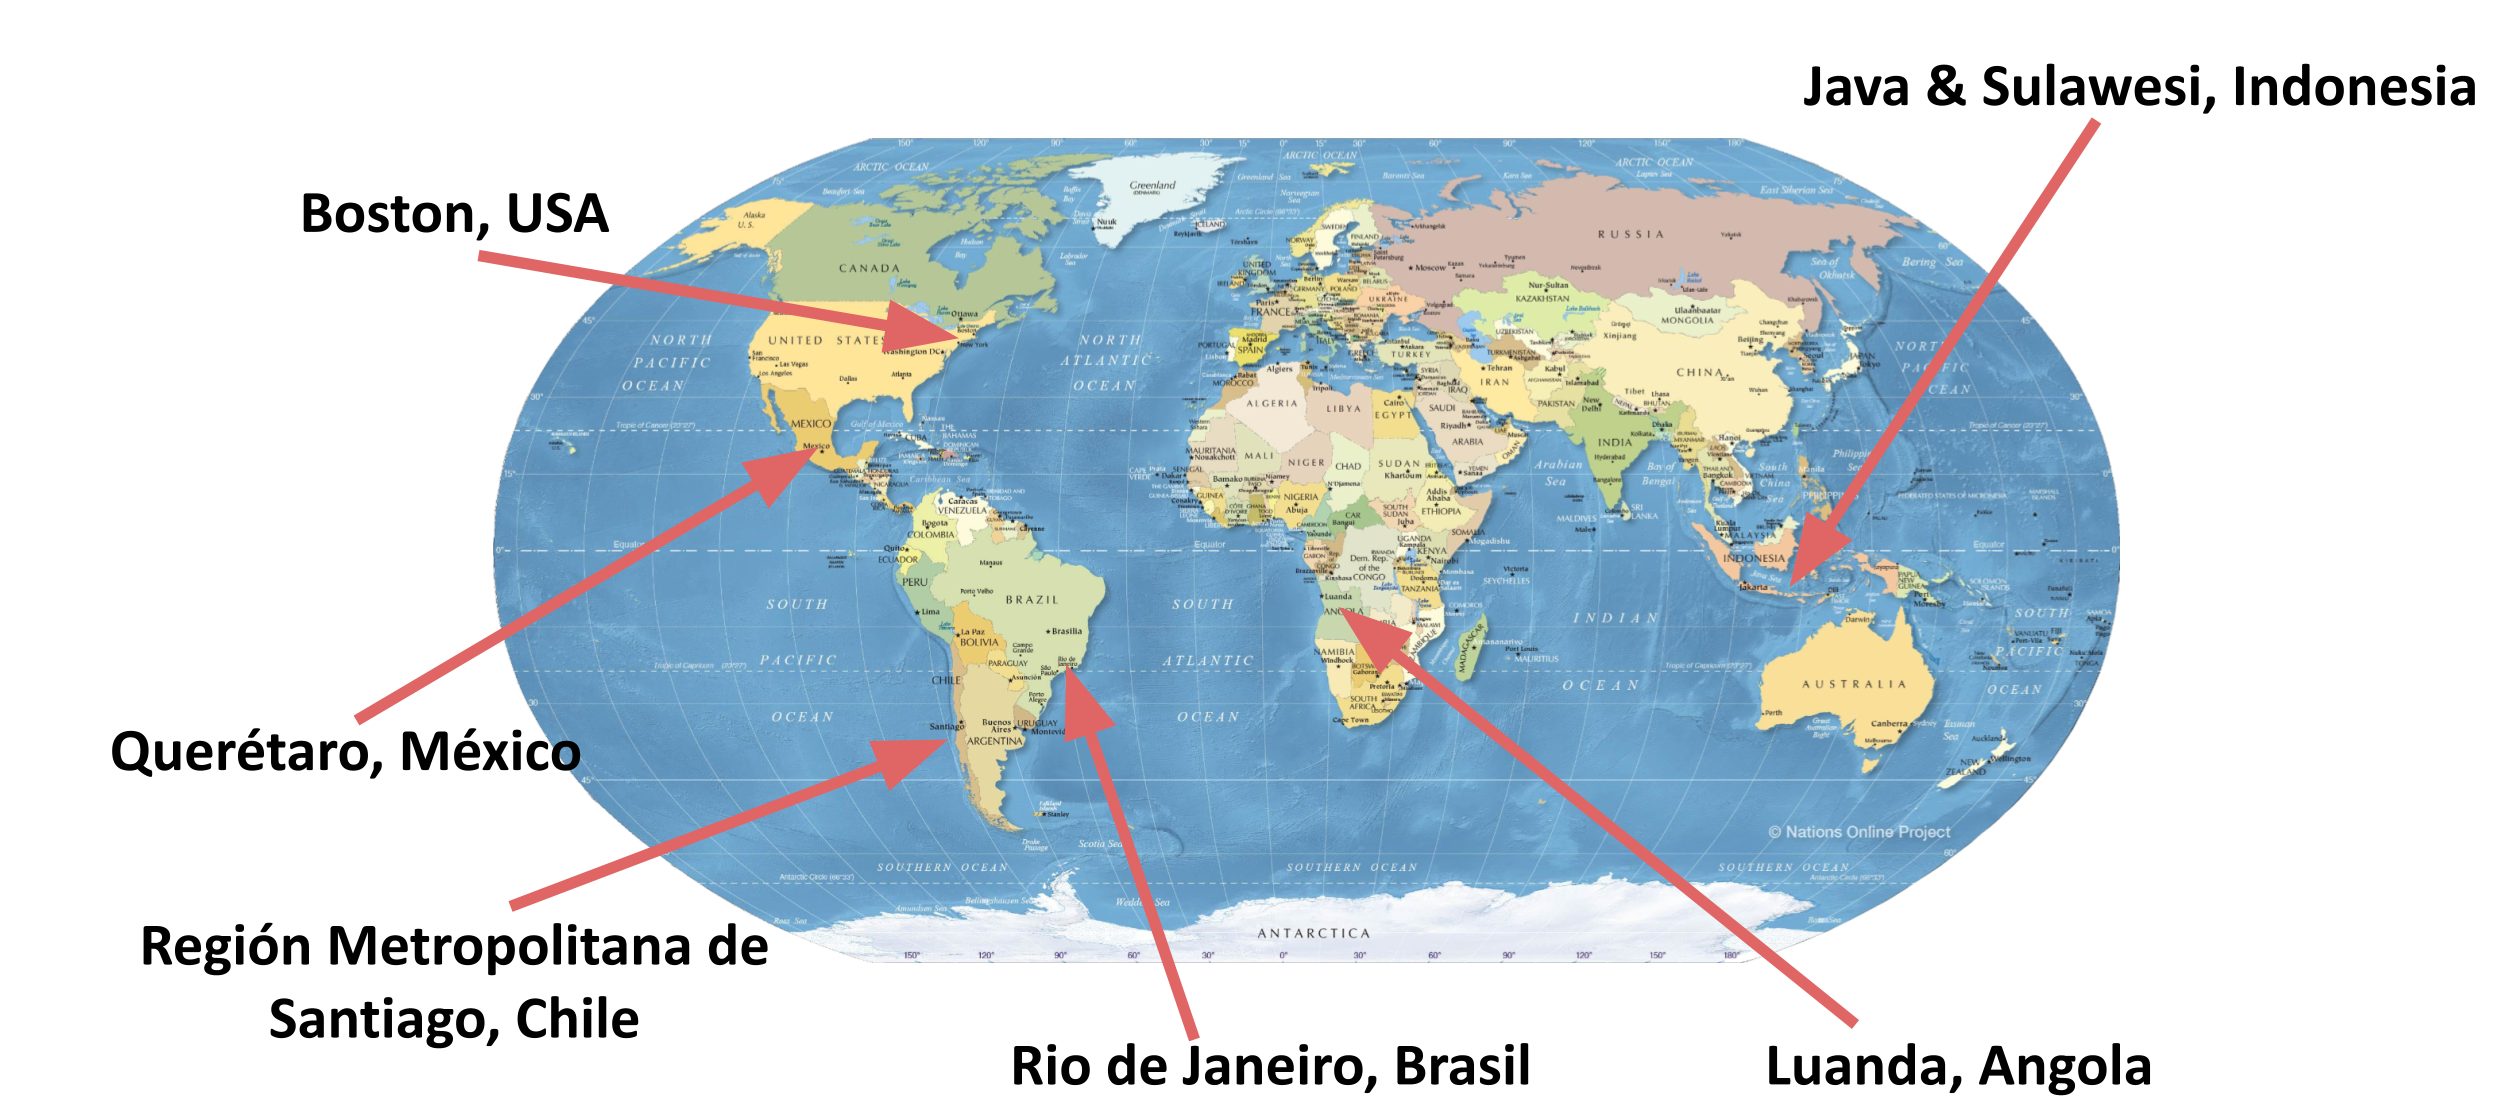
\includegraphics[width=0.9\textwidth]{Figures/chap5/vida_map.png}
	\caption{Areas participating in the Vida DSS International Network}
	\label{fig:vida_map}
\end{figure}

The system of interest for this case study is defined to include \ac{covid} response policymaking by the local or regional government, relevant aspects of the environment, and the general public in each of these areas. We do not consider the broader national or international aspects of the \ac{covid} pandemic, except where they intersect within each of these geographic areas (such as national Chilean social distancing policies applying to the Región Metropolitana de Santiago). 

Whereas the first case study focuses on simulating the changes in mangrove forest over decades, the focus of Vida is examining hourly to weekly air and water quality data alongside daily \ac{covid} epidemiological data and weekly quarantine policies. Government officials need actionable data to both address the ongoing public health crisis and to cope with the resultant socioeconomic and environmental consequences. Community members need to understand why their government is making the decisions that it is and understand the risks associated with their own actions.

It was beyond our resources (in both labor and time) to conduct the deep dive study of the System Context that was conducted in Chapter \ref{ch:mangroves} for each of the study areas. Instead, this examination focused on the commonalities across all of the areas, while still noting key differences with the potential to influence needs and objectives. 

%The analysis of System Context will include existing public health infrastructure in these metropolitan areas, how vulnerable they are to epidemics, and how decision-making occurs.	


\subsubsection{Analyze System Stakeholders}

The Technical Area Experts on this project included researchers from Harvard Medical School, \ac{nasa} Goddard Space Flight Center, and East Carolina University, as well as private consultants from Blue Raster. These individuals were recruited by Prof. Danielle Wood and myself specifically to fill gaps in the Space Enabled team's expertise.

Meanwhile the Local Area Experts (many of whom are technical experts in their own right) included a mix of government officials and academic researchers, most of whom work in the public health and/or in \ac{gis}. The government officials themselves span several different offices, including public health departments, data management authorities, science ministries, and space agencies. The list of primary Local Area Experts are shown in Table \ref{tab:vida_participants}. This does not include other individuals who participated more briefly, such as other members of these experts' respective organizations, hospital administrators, and \ac{ngo} representatives. These individuals joined in the Vida project in a variety of ways. Some, such as Felipe Mandarino of \ac{ipp} was already working with Space Enabled on an \ac{evdt} project (namely the Chapter \ref{ch:mangroves} case study). The onset of the pandemic caused those projects to pause or end and our collaborators asked if we could pivot to supporting \ac{covid} response, providing the initial impetus for the Vida project. Others, such as officials at Chile's \ac{minciencia} or Indonesia's Universitas Dipnegoro, we are corresponded with previously but had no ongoing projects with. When the pandemic started, either they contacted us or we contacted them (it varied from stakeholder to stakeholder) about joining in the Vida project.

The intended Users are those same individuals as well as the various public health agencies and task forces that they are affiliated with.  

\begin{table}[!htb]
\caption[Vida DSS International Network Participants]{Primary Vida \ac{dss} International Network participants.} \label{tab:vida_participants}
\begin{center}
\scriptsize
\begin{tabular}{|C{3cm}|C{3cm}|C{4cm}|} \hline
 
\textbf{Study Area} & \textbf{Name} & \textbf{Organization} \\ \hlinewd{2pt}

\multirow{3}{3cm}{Luanda} & Gilson Santos & \ac{ggpen} \\
& Eduina Teodoro & \ac{ggpen} \\
& Zolana Joao & \ac{ggpen} \\ \hline

Rio de Janeiro & Felipe Mandarino & \ac{ipp} \\ \hline

\multirow{2}{3cm}{Región Metropolitana} & Paulina Assmann & \ac{minciencia} \\
& José Guridi & \ac{minciencia} \\ \hline

\multirow{2}{3cm}{Java \& Sulawesi} & Hanifa Denny & Universitas Diponegoro \& the Indonesia Ministry of Health \\
& Joga Setiawan & Universitas Diponegoro \\ \hline

\multirow{2}{3cm}{Querétaro} & Joaquín Salas & \ac{ipn} \\
& Alejandro Monsiváis Huertero & \ac{aem} \\ \hline

\end{tabular}
\end{center}
\end{table}


Due to the urgent nature of the situation, no formal interviews were conducted at the beginning of the project, unlike the approach taken in Chapter \ref{ch:mangroves}. Instead, we relied upon a higher tempo of remote meetings to provide for quicker feedback. This included weekly or biweekly one-to-one meetings (Space Enabled researchers and representatives of one the metropolitan areas) and monthly multilateral meetings (including Technical Area Experts, Local Area Experts, and other guests from all of the metropolitan areas). These meetings allowed for local stakeholders to identify site-specific needs and thereby inform the \ac{dss} architecture; surface, provide, and integrate relevant data products, particularly those generated in-situ by government authorities; participate in the design and implementation of the \ac{dss} prototypes; and evaluate the prototypes. In general this resulted in a more iterative process than the fairly linear process depicted in Figure \ref{fig:evdt_framework}.

During the initial meetings each study area, we asked questions about the relationships between stakeholders, including how \ac{covid} policy decisions were made; immediate priorities for \ac{covid} response and more long-term concerns about the impacts of the pandemic; what datasets were available in their study area; what potential datasets and analyses were of most interest; and what characteristics of a \ac{covid} \ac{dss} were most important to them. These questions were regularly revisited during the future meetings, with responses often evolving over the course of the pandemic. In many cases, responses also changed due to seeing updates from other study areas during the monthly multilateral meetings.

In various cases, we worked with the Local Context Area Experts to schedule similar meetings with other stakeholders in the area, where similar questions would be asked.


\subsubsection{Understand Desired Outcomes \& Objectives}

While the initial overarching objective of the Vida project was to support effective decision-making in response to the \ac{covid} pandemic, there was still work to be done defining what exactly this entailed and how it varied from stakeholder to stakeholder. This was done iteratively. The Local Area Experts from each study area would identify specific Needs, Desired Outcomes, and potential System Objectives. They would also identify other stakeholders in their study area, who would in turn be contacted and involved in this process. They also helped gather core datasets for use in the Vida \ac{dss} (discussed further in Section \ref{sec:vida-evdt}). 

Various team members and I would then use these to develop analyses and improve the \ac{dss}. These would be presented to the Local Area Experts. They would then update and revise their needs based on these prototypes, on seeing similar prototypes for the other study areas, and on the dynamic nature of the pandemic. What I will present here is a synthesis from over the course of the project, rather than indicative of any particular point in time.

\subsubsection{Select System Functions}

System Functions were selected by considering the various Stakeholder Needs, Desired Outcomes, and System Objectives to identify where significant overlap existed. These were then compared with the feasibility of each function given available data and other resources, which varied from study area to study area.

In general, if formatted data was already readily available and a stakeholder expressed a preference for its inclusion, we added it to the \ac{dss} immediately. Custom analysis and additions to simulations required more effort by the Vida team and thus were typically only pursued for strong stakeholder preferences or for preferences that were common across multiple study areas.

\subsubsection{Assign Functions to Forms}

We assigned system Functions to Forms based on balancing the capabilities of the Space Enabled team with the needs and preferences of the stakeholders. The \ac{dss} and analyses were built upon existing expertise and code base from the \ref{ch:mangroves} case study, which both facilitated a rapid start but also brought along certain limitations. As needed, additional Technical Area Experts were enlisted to expand our capabilities. 

One key meta-objective was for the \ac{dss} to be designed such as to make it easy to add additional datasets, analysis results, and simulation components on a per-study-area basis. This enabled rapid revisions as stakeholders brought forward new potential functions as the pandemic developed (or abandoned old ones) or as analysis methods reached dead ends.

\subsubsection{Monitor and Evaluate Systems}

We cannot directly evaluate the impact of the Vida \acp{dss} on \ac{covid} response policy due to the infeasibility of comparing their use with counterfactual scenarios in which they were not used (not to mention the ethical concerns if this was possible). In the absence of a direct evaluation, we focused on perceived utility by the stakeholders and on general lessons learned from the analyses and \ac{dss} development process. This took the form of iterative reviews and improvements throughout the project lifespan. Within each component of the \ac{dss}, more particular forms of monitoring and evaluation were possible. For example in for the public health modeling component, simulated scenarios could be compared to actual case counts as the pandemic developed.

\subsection{SAF Results} \label{sec:vida-saf-result}

\subsubsection{System Context}

Both the impacts of \ac{covid} and the available means to respond to it are complicated and multi-faceted. Testing and vaccinations involve long, international supply chains. Medical treatment became an immense logistical problem as hospital beds and ventilators quickly reached capacity. Policy-makers found themselves making both public health decisions (such as social distancing, mask orders, and lockdowns) and economic measures (such as personal stimulus checks, increased unemployment benefits, and small business loans), the latter often seeking to mitigate the socioeconomic impacts of the former. Such impacts were considerable and diverse. Many places saw increases in unemployment, food insecurity, and housing cost burden, particularly for poorer or historically discriminated populations \cite{melnikGreaterBostonHousing2020}. Low-income children often rely upon free school meals and their parents rely upon said schools for daytime childcare. A transition to remote education threatened both \cite{nicolaSocioeconomicImplicationsCoronavirus2020}. Domestic abuse helplines saw an increase in calls during the pandemic lockdowns \cite{ivandicChangingPatternsDomestic2020}. 

To monitor and mitigate the spread of the pandemic, use of technologies for tracking, infection screening, contract tracing, and clinical management have also been developed and implemented \cite{whitelawApplicationsDigitalTechnology2020}. Policymakers and every day community members found themselves juggling complicated relationships between public health, the environment, socioeconomic factors, decision-making, and the new technologies necessary to monitor and respond to the pandemic. It is thus clear that the impacts of and responses to the pandemic can be characterized as a complex system, thus warranting the kind of multidisciplinary, model-based approach of which \ac{evdt} is an example \cite{deweckHandlingCOVID192020}.

The study areas themselves varied quite significantly in their response to the \ac{covid} pandemic, their preparedness for such events, and their vulnerability to is impacts. They also vary in more basic characteristics such as geographic size and population. Table \ref{tab:vida_area_stats} summarizes some basic facts about these cities. These differences, which vary by more than an order of magnitude in some cases, illustrate that the concerns, priorities, and decision-making processes are also likely to differ significantly from location to location, though they are united by a common desire to effectively respond to the \ac{covid} pandemic.

\begin{table}[!htb]
\caption[Vida Study Area Statistics]{Basic facts and statistics for each of the Vida study areas. All statistics are from their respective national statistical agency and may not be for precisely the same years as one another. The term \textit{province} is here used to refer to the administrative unit just smaller than that of the country. The actual term for this kind of unit varies from country to country. \textsuperscript{a} Statistics shown in this table are aggregated from the provinces of West Java, Central Java, East Java, Jakarta, and South Sulawesi. \textsuperscript{b} This figure is for the nation of Angola as I could not find reliable information for the Luanda metropolitan area.} \label{tab:vida_area_stats}
\begin{center}
\scriptsize
\begin{tabular}{|C{1.75cm}|C{1.75cm}|C{1.5cm}|C{1cm}|C{1.5cm}|C{1.5cm}|C{1cm}|C{1.5cm}|} \hline
 
\textbf{Study Area} & \textbf{Scale} & \textbf{Population (M)} & \textbf{Size (km2)} & \textbf{Population Density} & \textbf{Nominal GDP per Capita (\$)} & \textbf{Coastal Port} & \textbf{Capital} \\ \hlinewd{2pt}

Luanda, Angola & Metropolitan Area / National & 8.33 & 1876 & 4440 & 3997\textsuperscript{b} & X & National \\ \hline
Rio de Janeiro, Brazil & Municipality & 6.75 & 1221 & 5528 & 11032 & X & Provincial \\ \hline
Región Metropolitana de Santiago, Chile & Province & 7 & 15403 & 454 & 13466 & & National \\ \hline
Java \& Sulawesi\textsuperscript{a}, Indonesia & Multi-Provincial & 144.99 & 163360 & 888 & 4593 & X & National \\ \hline
Querétaro, Mexico & Province & 2.37 & 11699 & 203 & 9179 & & \\ \hline
Boston, USA & Metropolitan Area & 4.94 & 11700 & 422 & 83597 & X & Provincial \\ \hline
\end{tabular}
\end{center}
\end{table}

Each of these areas had other assets and obstacles not easily seen in such bulk statistics. Brazil in general, and Rio de Janeiro in particular, has robust and historically successful public vaccination infrastructure. Nonetheless, troubled by misinformation and federal mismanagement, this process did not go near so smoothly during this pandemic \cite{ferreiraEstimatingImpactImplementation2023}. The Boston area contains numerous medical research institutions, some of whom were able to retool to providing community \ac{covid} testing for the region \cite{eisenstadtHowBroadInstitute2020}. Chile's had a Ministry of Science that was prepared to serve as the coordinator for numerous datasets \cite{ministeriodecienciatecnologiaconocimientoeinnovacionDatosCOVID192021} and to quickly create a wastewater testing system \cite{gallardo-escarateWastewaterMicrobiomeNovel2021}.

The decision-making processes varied across the study areas as well. Some areas left significant latitude to municipal or provincial decision-makers. This was the case for Rio de Janeiro, for instance, was able to set many closure and reopening policies at the municipal level. Others, such as Luanda, set most policies at the national level. 

In general, the differences between study areas pointed us towards a need for normalization in order to enable comparison across study areas (this is discussed further in Section \ref{sec:vida-evdt-method}). Commonalities were used to prioritize System Functions later in the \ac{saf} process. For instance, the fact that four of the six study areas were coastal ports suggested that the Luanda stakeholders' expressed interest in tracking ships in the harbor (presented in these \ac{saf} results) may relevant to other stakeholders as well.

Figure \ref{fig:dimensions_vida} summarize the commonalities among the study areas as these are what guided much of the Vida development process.

\begin{figure}[!htb] 
\centering
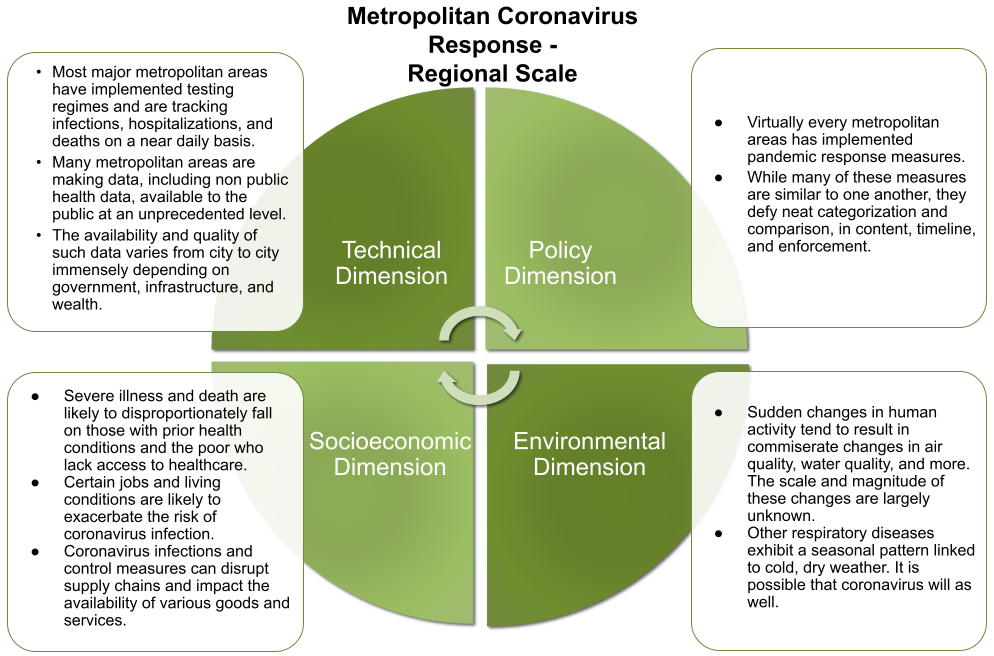
\includegraphics[width=0.8\textwidth]{Figures/chap5/dimensions_vida.png}
\caption[Vida System Context Dimensions]{Vida System Context Dimensions}
\label{fig:dimensions_vida}
\end{figure}


\subsubsection{Analyze System Stakeholders} \label{sec:vida-saf-stakeholders-result}

Analyzing the relationships between stakeholders in this case study posed some challenges particular to this situation. While some generalizations can be made across the study areas (e.g. policies on international travel were set by national government agencies; \ac{covid} response policies tended to involve some combination of mask mandates and closures of public spaces), there was significant variation between the study areas in how decisions were made and who made them. This was both due to differences in the underlying political structure of the study areas (in some, decisions are made primarily centrally and in others decisions are more decentralized) and to the fact that the \ac{covid} pandemic upended normal decision-making processes. These were replaced by much more dynamic and distributed decision-making relationships that involved much of society in one way or another. This can be glimpsed even in the Table \ref{tab:vida_participants} list of direct Vida participants, which includes health, science, and space ministries, among others.

For this reason, even a detailed, stationary stakeholder relational map for each particular study area would contain inaccuracies and over simplifications. Instead, I opted for a basic primary-secondary-tertiary classification of stakeholders, as seen in Figure \ref{tab:vida-stakeholders}, that focuses on the Vida project, rather than \ac{covid} decision-making as a whole. 

\begin{table}[!htb]
\caption[Vida Stakeholders]{Primary-Secondary-Tertiary classification of Vida stakeholders}
\label{tab:vida-stakeholders}
\begin{center}
\scriptsize
\begin{tabular}{ L{4cm} L{4cm} L{4cm} } \hline

\textbf{Primary} & \textbf{Secondary} & \textbf{Tertiary}  \\ \hline

\tabitem{Public Health Policymakers}  & \tabitem{US Vida Team} & \tabitem{General public in each study area} \\
 
\tabitem{Vida International Network Participants} & \tabitem{Other government agencies involved in \ac{covid} response} & \tabitem{Healthcare providers} \\ \hline
\end{tabular}
\end{center}
\end{table}

It is also worth noting that the Local Context Area Experts listed previously in Table \ref{tab:vida-stakeholders} vary in their relationship with direct \ac{covid} decision-making authority. 

\begin{enumerate}[itemsep=0pt,parsep=0pt]
    \item{\textbf{Luanda, Angola - \ac{ggpen}:} Angola's space agency provides useful data and analysis to decisionmakers but was not directly involved in the \ac{covid} policymaking themselves or in its presentation to the public.}  
    \item{\textbf{Rio de Janeiro, Brazil - \ac{ipp}:} The municipal data science agency provides useful data and analysis to decisionmakers but was not directly involved in the \ac{covid} policymaking. They were, however directly involved with presenting information on policies and on the current state of the pandemic to the public via online dashboards and the publication of data.}
    \item{\textbf{Región Metropolitana de Santiago, Chile - \ac{minciencia}:} The national science agency was not directly involved in the \ac{covid} policymaking themselves, but they were formally assigned responsibility for generating and collating all pandemic-related data for use by various government agencies and by the public. They were also given responsibility for generating insights from this data themselves.}
    \item{\textbf{Java \& Sulawesi, Indonesia - Universitas Diponegoro \& the Indonesia Ministry of Health}: The former of these served in an advisory role to the latter, which was directly involved with setting \ac{covid} policy across the country.}
    \item{\textbf{Querétaro de Arteaga, Mexico - \ac{ipn} \& \ac{aem}:} Both of these organizations played an advisory role in decision-making, the former primarily on the provincial level and the latter primarily on the national level.} 
\end{enumerate}

As can be seen above, the Local Context Area Experts are largely not the primary creators or enforcers of \ac{covid} response policies in their respectively study areas. At the same time, they have significantly more influence on those policies than the average member of the community. They also sit in a variety of different kinds of organizations. Each of these factors likely influenced the priorities that they expressed. We kept this in mind when analyzing the Desired Outcomes and Objectives below.

\subsubsection{Understand Desired Outcomes \& Objectives}

Over the course of the Vida International Network collaboration, a wide variety of Stakeholder Needs, Desired Outcomes, and potential \ac{dss} System Objectives were surfaced. Table \ref{tab:vida-needs} summarizes the more common and continuous preferences. It should be noted that while these preferences were based on both the Local Context Area Experts and other stakeholders in each study area, the former had the most sustained and direct opportunities to express preferences, so the table disproportionately represents their views. As such, the particular circumstances of each of these experts, discussed just previously during the stakeholder analysis, must be kept in mind.

Significant overlap can be seen across the stakeholders, but so too can certain differences, particularly in the System Objectives column. In general, stakeholders expressed the need for the ability to visualize multiple different kinds of data and understanding the relationships between them, including future looking. Most of the study areas quickly began collecting and publishing pandemic-related data, both directly tied to public health and more distantly related to the pandemic (e.g. \cite{ministeriodecienciatecnologiaconocimientoeinnovacionDatosCOVID192021}). Some even maintained interactive visualizations of \ac{covid} cases and hospitalizations (e.g. \cite{rioprefeituraPainelRioCOVID192020}). In general, however, they lacked visualizations capable of showing the public health status along side other factors such as socioeconomic impacts/vulnerability, environmental effects and risk factors, and future projections.

This provided enough alignment to pursue a shared foundation moving forward, with particular datasets and analyses to be customized to the Needs and Desired Outcomes of each study area.

\begin{landscape}
\scriptsize
\begin{longtable}{| C{2cm} |  L{5.2cm} | L{5.2cm} | L{5.2cm} |}
\caption[Needs, Outcomes, and Objectives for Rio de Janeiro Case Study]{Stakeholder Needs, Desired Outcomes, and potential System Objectives for key stakeholders in the Rio de Janeiro Case Study}
\label{tab:vida-needs} \\ \hline
\textbf{Study Area} & \textbf{Stakeholder Needs} & \textbf{Desired Outcomes}  & \textbf{Potential \ac{dss} System Objectives} \\ \hlinewd{2pt} \endfirsthead

\hline \textbf{Study Area} & \textbf{Stakeholder Needs} & \textbf{Desired Outcomes}  & \textbf{Potential \ac{dss} System Objectives} \\ \hlinewd{2pt} \endhead

\multirow{4}{2cm}{\centering Luanda} & \tabitem{Minimize deaths and other serious health consequences of the pandemic} & \tabitem{Limit the spread of \ac{covid}} & \tabitem{Support closure policy decision-making} \\ 
 & \tabitem{Minimize negative economic consequences of the pandemic} & \tabitem{Provide proper treatment for \ac{covid} cases} & \tabitem{Monitor and analyze air quality and fires in the region} \\ 
& \tabitem{Understand the dynamics and impacts of \ac{covid}} & \tabitem{Keep supply chains operational} & \tabitem{Monitor and analyze changes in ship traffic in Luanda Bay} \\ 
& & \tabitem{Know how the pandemic will evolve and change in the coming days, weeks, and months} & \tabitem{Forecast \ac{covid} cases and their impacts} \\ \hline
 
\multirow{4}{2cm}{\centering Rio de Janeiro} & \tabitem{Minimize deaths and other serious health consequences of the pandemic} & \tabitem{Limit the spread of \ac{covid}} & \tabitem{Support closure policy decision-making} \\ 
 & \tabitem{Minimize negative economic consequences of the pandemic} & \tabitem{Provide proper treatment for \ac{covid} cases} & \tabitem{Monitor and analyze air quality in the region} \\ 
& \tabitem{Understand the dynamics and impacts of \ac{covid}} & \tabitem{Know how individuals are responding to \ac{covid} policies} & \tabitem{Monitor and analyze changes in human activity and mobility} \\ 
& & \tabitem{Know how the pandemic will evolve and change in the coming days, weeks, and months} & \tabitem{Forecast \ac{covid} cases and their impacts} \\ \hline

\multirow{5}{2cm}{\centering Metropolitana} & \tabitem{Minimize deaths and other serious health consequences of the pandemic} & \tabitem{Limit the spread of \ac{covid}} & \tabitem{Support closure policy decision-making} \\ 
 & \tabitem{Minimize negative economic consequences of the pandemic} & \tabitem{Provide proper treatment for \ac{covid} cases} & \tabitem{Monitor air quality in the region} \\ 
& \tabitem{Understand the dynamics and impacts of \ac{covid}} & \tabitem{Know how individuals are responding to \ac{covid} policies} & \tabitem{Monitor and analyze changes in human activity and mobility} \\* 
& & \tabitem{Know how the pandemic will evolve and change in the coming days, weeks, and months} & \tabitem{Forecast \ac{covid} cases and their impacts} \\* 
& & & \tabitem{Visualize and analyze already published data in the \ac{covid} repository} \\ \noalign{\penalty-5000} \hline

\multirow{1}{2cm}{\centering Java \& Sulawesi} & \tabitem{Minimize deaths and other serious health consequences of the pandemic} & \tabitem{Limit the spread of \ac{covid}} & \tabitem{Support closure policy decision-making} \\* 
 & \tabitem{Minimize negative economic consequences of the pandemic} & \tabitem{Provide proper treatment for \ac{covid} cases} & \tabitem{Visualize and monitor changes over multiple distinct areas} \\* 
& \tabitem{Understand the dynamics and impacts of \ac{covid}} & \tabitem{Know how individuals are responding to \ac{covid} policies} & \tabitem{Monitor and analyze changes in human activity and mobility} \\* 
& & \tabitem{Know how the pandemic will evolve and change in the coming days, weeks, and months} & \tabitem{Forecast \ac{covid} cases and their impacts} \\*
& & \tabitem{Know what economic consequences the pandemic is causing} & \tabitem{Monitor and analyze a variety of economic impacts of the pandemic} \\  \hline

\multirow{1}{2cm}{\centering Querétaro} & \tabitem{Minimize deaths and other serious health consequences of the pandemic} & \tabitem{Limit the spread of \ac{covid}} & \tabitem{Support closure policy decision-making} \\ 
 & \tabitem{Minimize negative economic consequences of the pandemic} & \tabitem{Provide proper treatment for \ac{covid} cases} & \tabitem{Monitor and analyze changes in human activity and mobility} \\ 
& \tabitem{Understand the dynamics and impacts of \ac{covid}} & \tabitem{Know how the pandemic will evolve and change in the coming days, weeks, and months} & \tabitem{Forecast \ac{covid} cases and their impacts} \\ \hline

\end{longtable}

\end{landscape}


\subsubsection{Select System Functions}

Based on the above analysis, several \ac{dss} system functions were selected. These are:

\begin{itemize}[itemsep=0pt,parsep=0pt]
	\item{\textbf{Visualize historical public health data and relevant data.} The public health data includes \ac{covid} cases, deaths, and hospitalizations, among others. The relevant non-public-health data is based on the priorities of each study area but include such things as \ac{covid} response policy decisions, air quality, economic indicators, and mobility data.}
	\item{\textbf{Identify and highlight connections between public health and non-public-health phenomena.} These can go in either direction, such as the impact of weather and air quality on the infectiousness of \ac{covid} or the impact of \ac{covid} on jobs.}
	\item{\textbf{Simulate potential future trajectories of the pandemic based on different policy decisions.} True forecasting was deemed to be beyond the capabilities of this team, but scenario generation was considered an acceptable alternative for raising the potential implications of different policy choices.} 
\end{itemize}

Each of the above further the overall goal of decision-makers in each of the study areas to mitigate the impacts of \ac{covid}. The specific topics of analysis and elements to be included in the \ac{dss} represent what stakeholders found most relevant to that goal.

In addition to these \ac{dss}-specific functions, there were some additional functions to be performed by the Vida International Network as a whole, namely:

\begin{itemize}[itemsep=0pt,parsep=0pt]
	\item{\textbf{Share information on \ac{covid} response across participants.} Analyses undertaken for a particular study area may turn out to be relevant to another. Additionally, independent of the Vida project, each study area was experimenting with a variety of response measures. The successes and failures of these measures constitute useful information for other participants.}
	\item{\textbf{Build capacity for multidisciplinary analysis and visualization.} This is useful beyond the \ac{covid} pandemic and the Vida International Network constitutes an opportunity for participants to learn from each other in this regard, in addition to the benefits of developing the Vida \ac{dss}.}
\end{itemize}

\subsubsection{Assign Functions to Forms}

In order to implement the \ac{dss} functions, two distinct forms were selected to be developed in parallel. The first was a desktop-based tool, based upon the design and code base of the \ac{dss} from Chapter \ref{ch:mangroves}. This was chosen primarily to facilitate the quick start to prototyping that was required by the urgency of the situation. It also ensured that the code and its assets were open-source and freely available, an important factor as the ability to pay varied from stakeholder to stakeholder. Finally, the familiarity with existing \ac{gis} software varied immensely from stakeholder to stakeholder, with some coming from completely different fields. There was thus less of a pressure to adopt an existing software platform, particularly since the situation was so novel as to not have much in the way of existing procedures to disrupt. This form, along with the overall \ac{saf} results, are summarized in Figure \ref{fig:vida-architecture}.

The other, parallel form was an online tool based in ArcGIS Online. Due to the limitations of the platform, it would focus on data visualization and would lack any scenario generation capability. This tool was developed primarily by Blue Raster, with members of the Space Enabled team (including myself) providing direction and certain datasets. Unlike the desktop version, which pursued each of the study areas simultaneously and in parallel, the online version would be developed for study areas sequentially, starting with a Boston area prototype.

The primary form to address the non-\ac{dss} functions were multilateral meetings in which all of the participants could share lessons and information. These are discussed further in Section \ref{sec:vida-collab}.


\begin{figure}[!htb]
	\centering
	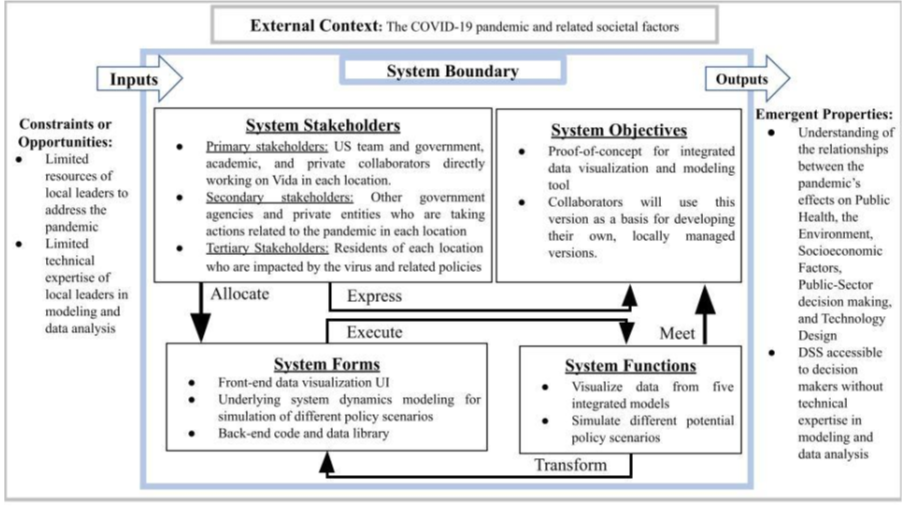
\includegraphics[width=1\textwidth]{Figures/chap5/architecture.png}
	\caption{The high-level functional systems architecture of the Vida \ac{dss}.}
	\label{fig:vida-architecture}
\end{figure}

\subsubsection{Monitor and Evaluate Systems}

The monitoring and evaluation of the Vida \acp{dss} were highly iterative, with stakeholders regularly surfacing new needs and new datasets to help address those needs. Various threads would be proposed, investigated, and then abandoned if they did not prove to be feasible or useful. Several of these are mentioned throughout \ref{sec:vida-evdt} as they come up. A more wholistic evaluation of the entire Vida project takes place in Section \ref{sec:vida-discuss}.

\section{EVDT Application} \label{sec:vida-evdt}

The following subsections walk through the components of the system from an \acf{evdt} perspective, detailing what models were used and the results of those models. Before proceeding though, it is worth stating what exactly each of the four components of \ac{evdt} mean for this system. The onset of the COVID-19 pandemic was an immensely significant event around the world. Thus, while it would have been possible to consider public health as a component of the Vulnerability model, in order to properly center and prioritize the public health aspects of the pandemic, a dedicated Public Health Model was added to the default \ac{evdt} arrangement, as shown in Figure \ref{fig:vida_flow}. 

In order to select what to include in each of the \ac{evdt} models, we must return to the earlier identified System Functions:

\begin{itemize}[itemsep=0pt,parsep=0pt]
	\item{\textbf{Visualize historical public health data and other relevant data.}}
	\item{\textbf{Identify and highlight connections between public health and non-public-health phenomena.}}
	\item{\textbf{Simulate potential future trajectories of the pandemic based on different policy decisions.}} 
\end{itemize}

The first two are closely tied together and must be grounded in the Stakeholder Needs, Desired Outcomes, and System Objectives note in Table \ref{tab:vida-needs}. Public Health has the most commonality across stakeholders. Each were heavily invested in understanding how case counts, hospitalizations, mortality, and infection rates change over time. These would also be the primary focus of the third of the above functions.

Interest in various non-public-health phenomena had both more variation across study areas and less confidence within each study area. The relevance of such factors as air quality or water quality was unknown but remained a concern. There was also significant variation across study areas regarding the types of data available. Initial discussions with the Local Context Area Experts, other local stakeholders, and the Technical Area Experts, resulted in certain specific areas to be prioritized for initial investigation. More detail on the methods and results of each of these areas is provided in the following subsections.

\textbf{Environment:} Initial research by Mohammad Jalali, one of our Technical Area Experts, indicated that both weather and air quality could have an impact on the transmission of \ac{covid} \cite{xuModestImpactWeather2020}. We thus chose to investigate how air quality was changing over the course of the pandemic and which parts of each study area were likely to have worse air quality. In some areas, in-situ, station-based data was available while others had to rely only upon \ac{eo} satellite data.

\textbf{Vulnerability:} Stakeholders in each of the study areas were highly interested in the socioeconomic impacts that the pandemic and the various \ac{covid} response policies would have on the public. We chose to approach this in two parallel ways. One was to conduct qualitative surveys of members of the public. The other was to study how human activity and mobility was changing over the course of the pandemic.

\textbf{Decision-making:} The primary form of decision-making that stakeholders were interested in was \ac{covid} mitigation policies, such as mask mandates, public space closures, and travel restrictions. We tracked these policies over time, developed ways of comparing one study area to another, and studied what impact these policies had on both public health metrics and on human activity, namely mobility.

\textbf{Technology:} While \ac{eo} data was used in the above analyses, the primary relevant technology to stakeholders was \ac{covid} testing. Where available, we tracked data on rates of \ac{pcr} testing, but ultimately did not conduct any significant analysis. Possibilities for future work on this front are discussed later.

Returning to the four questions from Section \ref{sec:evdt-questions} (plus one additional one), we can summarize the above by asking the following:

\begin{enumerate}[itemsep=0pt,parsep=0pt]
	\item \textbf{What is happening in in public health?} How is the COVID-19 pandemic spreading through the community? What portion of the infected are being hospitalized or dying? What factors impact transmission?
	\item \textbf{What is happening in the natural environment?} How are air quality, water quality, and nightlights being altered by pandemic-related changes in human activity? What role does weather, smog, and other aspects of the environment have on COVID-19 transmission and symptoms?
	\item \textbf{How will humans be impacted by what is happening in the natural environment and in public health?} Who is at most risk of falling ill or suffering from severe symptoms? How are pandemic response policies affecting different populations? Do pandemic-related changes in air quality have a noticeable impact on the residents of these metropolitan areas? How are different industries impacted by such sudden changes in both supply and demand?
	\item \textbf{What decisions are humans making in response to environmental factors and why?} What are the different forms of pandemic response measures being taken by governments, both local and national? How are individual people altering their patterns of work, shopping, and recreation?  
	\item \textbf{What technology system can be designed to provide high quality information that supports human decision making?} What testing regime is needed to effectively reduce the spread of the virus and resultant deaths? What other data sources are useful for informing decision-making?
\end{enumerate}

It should be noted that, unlike in the Chapter \ref{ch:mangroves} case study, there is no single through-line that connects each of these analyses and models. Instead a number of pairwise relationships exist. The impact of air quality on \ac{covid} and vice versa. The relationship between mobility and \ac{covid} or closure policies and mobility. As will be noted in the following subsections, there were also a variety of other investigations that were abandoned due to lack of stakeholder interest, reached some dead end, or were only relevant to a particular study area. The reasons for this were discussed in Section \ref{sec:vida-purpose} of this chapter and its implications are discussed in Section \ref{sec:vida-discuss}.

\begin{figure}[!htb]
	\centering
	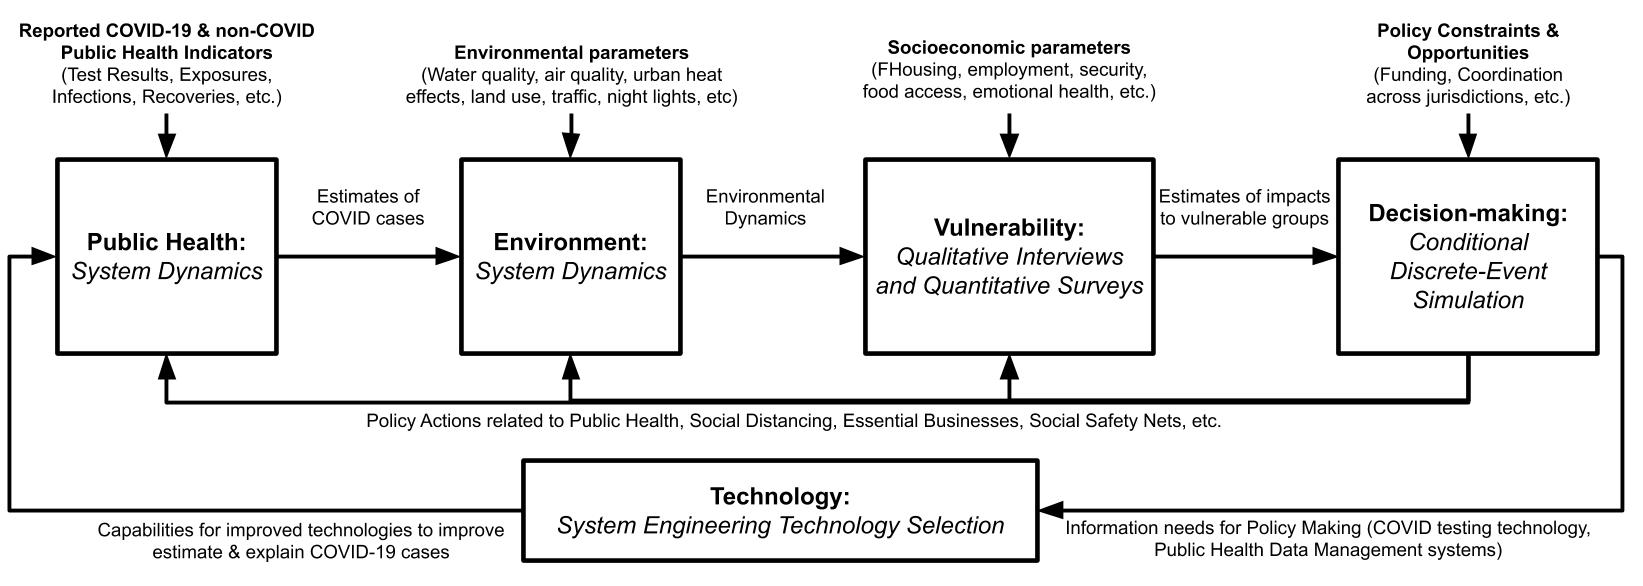
\includegraphics[scale=0.25]{Figures/chap5/Vida_Flowchart_v2.jpg}
	\caption[The Vida Variant of the EVDT Model]{The Vida variant of the EVDT model, designed to support decision making by governments during COVID-19}
	\label{fig:vida_flow}
\end{figure}

\subsection{EVDT Methodology} \label{sec:vida-evdt-method}

For each of the \ac{evdt} components (including the additional Public Health component), two levels of analysis were being conducted. At one level, we studied the relationship between different phenomena within each location to better understand how the pandemic was evolving in say Rio de Janeiro in particular. At the second level, we were studying phenomena across the different participating study areas, to understand what lessons were generalizable (and which were not). 

For this second level, data was normalized in various ways to facilitate comparison. Generally the state date for post-pandemic ($t=0$) was set at the date of first confirmed \ac{covid} case in each location. These correspond to (in order of occurrence):

 \begin{itemize}[itemsep=0pt,parsep=0pt]
	\item{Querétaro, Mexico: 10/Feb/2020}
	\item{Metropolitana, Chile: 04/Mar/2020}
	\item{Rio de Janeiro, Brazil: 07/Mar/2020}
	\item{Jakarta, Indonesia: 19/Mar/20}
	\item{Angola: 20/Mar/2020}
\end{itemize}

Similarly any statistic usually measured in "number of people" (such as \textit{new cases of \ac{covid} per day}) were normalized into per-capita values, based on the population of that location. Various other, more particular, forms of normalization (such as for \ac{covid} response policies) are discussed in their respective sections below.

Table \ref{tab:vida_data} provides a summary of the common data types across the study areas. The following subsections describe how they datasets are used in more detail.

\begin{table}[!htb]
\caption[Common Vida Data Types]{Common Vida data types} \label{tab:vida_data}
\begin{center}
\scriptsize
\begin{tabular}{|C{3cm}|C{6cm}|} \hline

\multirow{4}{3cm}{Public Health} & \tabitem{Coronavirus cases (active \& cumulative)} \\
& \tabitem{Hospitalizations and/or ICU occupancy} \\
& \tabitem{Coronavirus-attributed deaths} \\
& \tabitem{Case recoveries} \\ \hline

\multirow{2}{3cm}{Environment} & \tabitem{Air quality (particular matter, NOx, CO, etc.)} \\
& \tabitem{Urban nightlights} \\ \hline

\multirow{3}{3cm}{Socioeconomic Impacts} & \tabitem{Local \& national unemployment rates} \\
& \tabitem{Air and ship traffic} \\
& \tabitem{Intra-urban mobility rates \& patterns} \\ \hline

\multirow{2}{3cm}{Public Policy} & \tabitem{Business \& public activity closures and restrictions} \\
& \tabitem{Individual social distancing \& mask requirements} \\ \hline

\multirow{3}{3cm}{Technology Development} & \tabitem{Daily testing capacity} \\
& \tabitem{Ventilator availability} \\
& \tabitem{Sensing technology access} \\ \hline
\end{tabular}
\end{center}
\end{table}


Finally, much of this analysis focused on the first year of the pandemic, roughly early March of 2020 to early March of 2021.

\subsubsection{Environment} \label{sec:vida-evdt-e-method}

Unlike the previous case study, which focused on a particular aspect of the environment (mangroves) that had an established literature, the onset of the COVID-19 pandemic resulted in many disparate impacts on the environment in quick succession. Air quality noticeably improved as traffic patterns changed and work-related emissions declined \cite{isaifanDramaticImpactCoronavirus2020}. In many places, water quality noticeable improved and noise diminished \cite{aroraCoronavirusLockdownHelped2020}. As discussed earlier, it also was not immediately clear what topics were the highest priority to stakeholders. As a result, many areas were explored and only some pursued in detail. For the purposes of this thesis, I will focus on a subset of the air quality analysis that we conducted.

For this, we primarily relied upon in-situ data from MonitorAr stations in Rio de Janeiro  and the Sistema de Información Nacional de Calidad del Aire stations in the Santiago area , though we also used Sentinel-5P \ac{tropomi} data. In Rio de Janeiro, these sensors take hourly measurements to monitor a range of air quality parameters (e.g O3, CO, SO2, PM10, etc.) in 8 different barrios, or neighborhoods, of Rio de Janeiro. The dataset is provided publicly and freely through Rio de Janeiro's Data.Rio website and data stretches back to 2011 \cite{institutopereirapassosDadosHorariosMonitoramento2018}. In Chile, there are  11 sensors across the Metropolitana region, one each of several different municipalities, including Santiago. This data, which stretches back to 2010, was made available as part of the \ac{minciencia} \ac{covid} data repository on GitHub \cite{ministeriodecienciatecnologiaconocimientoeinnovacionDatosCOVID192021}.

With regards to the in-situ data, Maggie Zheng and I focused on changes in the measured PM10 pre-and-post pandemic. We process the data for each barrio by first calculating weekly averages to reduce intraweek variation, as we would expect there to be a difference in air emissions throughout the week (for instance, weekends versus weekdays). Then the data was fit using a least-squares estimate to a sinusoidal wave with an annual period. This sinusoidal curve is the average seasonal variation in PM10 for that barrio, and it is subsequently subtracted out from the data. A best-fit line is then calculated for this seasonally-corrected data. The best-fit line is long-term (multi-year) trend in PM10 measurements, and it is also subtracted out. At this point, the data is corrected for intraweek, seasonal, and annual trends, and we can then construct normalized histograms and statistically compare the pre-and-post pandemic distributions to identify changes and trends. 

In addition to these, there were several other environmental analyses conducted as part of this project, but not reported on in detail in this thesis. Amanda Payton used the Sentinel-5 \ac{tropomi} instrument to measure air quality (specifically SO2 and NO2) in the Luanda area and the \ac{modis} Daily Fire dataset to monitor changes in outdoor fires across the country. I did some initial investigation of the use of Landsat and Planet imagery for examining changes in water quality (particularly turbidity) in the water bodies adjacent to several of the study areas. Due to lack of interest from stakeholders, this was quickly abandoned and not pursued further.

\subsubsection{Public Health} \label{sec:vida-evdt-method-p}

The most notable variation that Vida has compared to previous \ac{evdt} applications is the addition of a dedicated Public Health Model. While the specific data collection definitions, coverage, and update cycles vary, each of the participant locations collected and published coronavirus-related epidemiological data on a regular basis, including newly identified infections, deaths, hospitalizations, etc. Vida ingests this data and uses it both to display historical trends alongside the other components and to conduct simulations of potential future behavior, with an emphasis on future trajectories of infections and hospitalizations. 

The Public Health component is based on a \ac{sir} system dynamics model. \ac{sir} is a compartmental epidemiological model and one of the most commonly used variants, due to its relative simplicity and flexibility. System dynamics is a modeling approach commonly used in both 'pure' epidemiological contexts \cite{homerSystemDynamicsModeling2006} and in broader public health policy contexts \cite{deutschCommunitybasedSystemDynamics2020}. Figure \ref{fig:vida_sd} shows a diagram depicting the layout of the Vida Public Health Model. In addition to the three traditional \ac{sir} components, it has two other health compartments: Hospitalizations and Deaths. These reflect some of the primary decision points and metrics of performance that policymakers are using. In most of our application contexts, population counts for each of these compartments is readily available on a daily or weekly basis. 

In the top left and bottom left of the diagram, the initial inclusions of Environment and Vulnerability components are shown. These are cursory and highly assumptive. Air pollutants, for example, are not merely a function of closure policy. In most locations that we have examined, and in research conducted by others \cite{isaifanDramaticImpactCoronavirus2020}, initial coronavirus-related closures resulted in a sudden drop of emissions (further discussion on this in the Section \ref{sec:vida-evdt-result}). Furthermore, there is some evidence that weather and air pollution have a modest impact on COVID-19 transmission \cite{xuModestImpactWeather2020}, leading to the inclusion of such an element in the top left of the diagram.

This model is non-spatial, though in some locations of interest with distinct geographies (such as the Indonesian islands of Java and Sulawesi), multiple independent instances of the model are generated.

\begin{figure}[!htb]
	\centering
	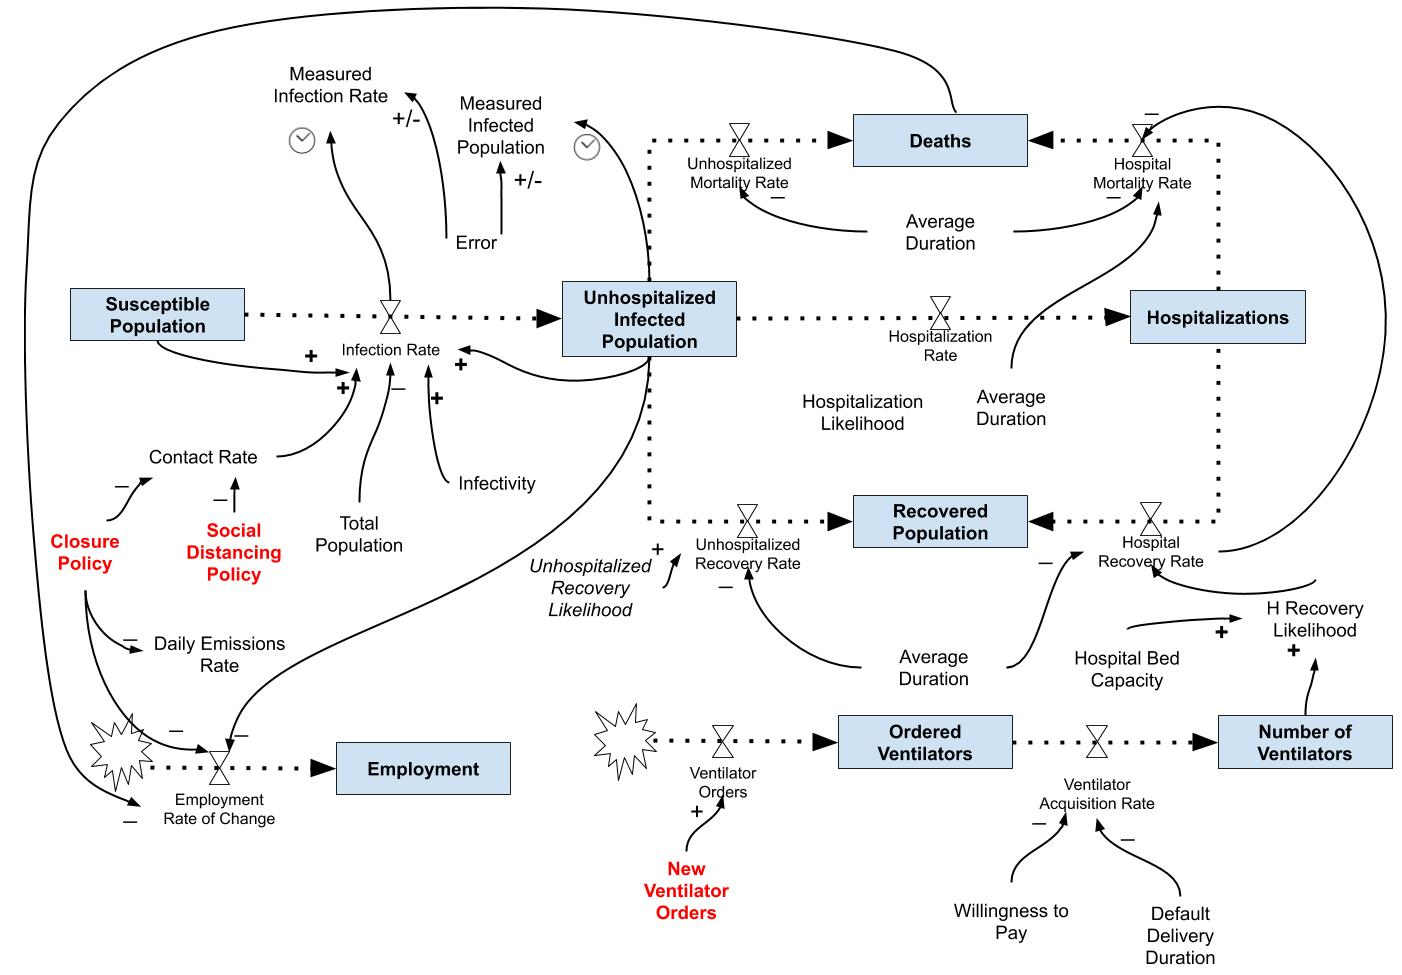
\includegraphics[scale=0.25]{Figures/chap5/SD_diagram.jpg}
	\caption[Current version of the Vida SIR system dynamics model]{Current version of the Vida \ac{sir} system dynamics model}
	\label{fig:vida_sd}
\end{figure}


\subsubsection{Vulnerability} \label{sec:vida-evdt-v-method}

Traditional, government-collected socioeconomic impact data largely does not exist at the fine temporal resolution required for coronavirus-related assessment during the early stages of the pandemic, so we had to develop the Invisible Variables Initiative (not discussed at length in this thesis) to work with our collaborators to develop surveys and interview procedures to elicit needed information. This initiative was led by Dr. Katlyn Turner and funded by the Natural Hazards Center at the University of Colorado, Boulder. 

As the pandemic progressed, however, some more traditional metrics, such as unemployment data, that show responses to the crisis began to be released and these were included in the \ac{dss}, but we did not conduct any significant analysis of them.

Another aspect of societal impact and vulnerability that Vida monitors is mobility. This includes movement as demonstrated by urban nightlights, telecommunications activity, automobile traffic, air traffic, and ship activity, the last of these primarily of relevance to the Luanda stakeholders. Telecommunications activity was made in numerous jurisdictions either directly by private companies \cite{googleCOVID19CommunityMobility} or via government data repositories \cite{ministeriodecienciatecnologiaconocimientoeinnovacionDatosCOVID192021} and integrated into Vida. The former of these also broke mobility into various kinds (residential, transit, recreational, etc.). This is important because it does not just matter how many trips individuals are making per day but also where they are going.

Telecommunications-based mobility data was tracked over time and compared to changes in closures policies (discussed further in the following Decision-making section). Other forms of mobility, such as air traffic passenger counts were included in the \ac{dss} but not significantly analyzed.

This mobility data however did not provide geographic specificity beyond province or nation. In order to provide more geospatial detail, we also examined urban nightlights, which were recognized to have changed and (generally) dimmed during the early phase of the pandemic \cite{elvidgeDimmingLightsChina2020}. We relied primarily on the \ac{viirs} VNP46A2 dataset \cite{romanNASABlackMarble2018}. This dataset contains daily panchromatic (visible and \ac{nir}) imagery at at a resolution of 15 arc-seconds (approximately 450m for the locations of interest) that have been corrected for atmospheric interference and moonlight variation. It is thus well suited for examining artificial lights, such as those generated by cities. We process it by masking out clouds and water (thereby eliminating transient lights from ships) using the supplied quality flag, then taking weekly median values to reduce intraweek variation, before calculating the relative anomaly compared to the 2019 median value for each pixel, thereby standardizing comparisons across time and space. Further normalization can be performed by identifying any long term trend from Jan 1st, 2019 to March 1st, 2020 (the approximate start of the pandemic) and subtracting this extrapolated trend from the post-pandemic data. Once this has been completed, we can calculate the Theil-Sen trend estimator for each pixel to determine the trend in nightlights during the initial phases of the pandemic.

We also statistically compare specific pre-and-post pandemic time periods at the various areas of interest to identify changes. In particular we performed a t-test to determine if a statistically significant difference exists between the pre-pandemic (January 2019 - Feb 2020) values and the post-pandemic (March 2020 - August 2020), calculated Pearson correlation coefficient to determine if there is a linear fit between the two periods and its directionality, and calculated the Theil-Sen trend estimator for both periods.

This methodology is summarized below in Figure \ref{fig:nightlights_method}.

\begin{figure}[!htb]
\centering
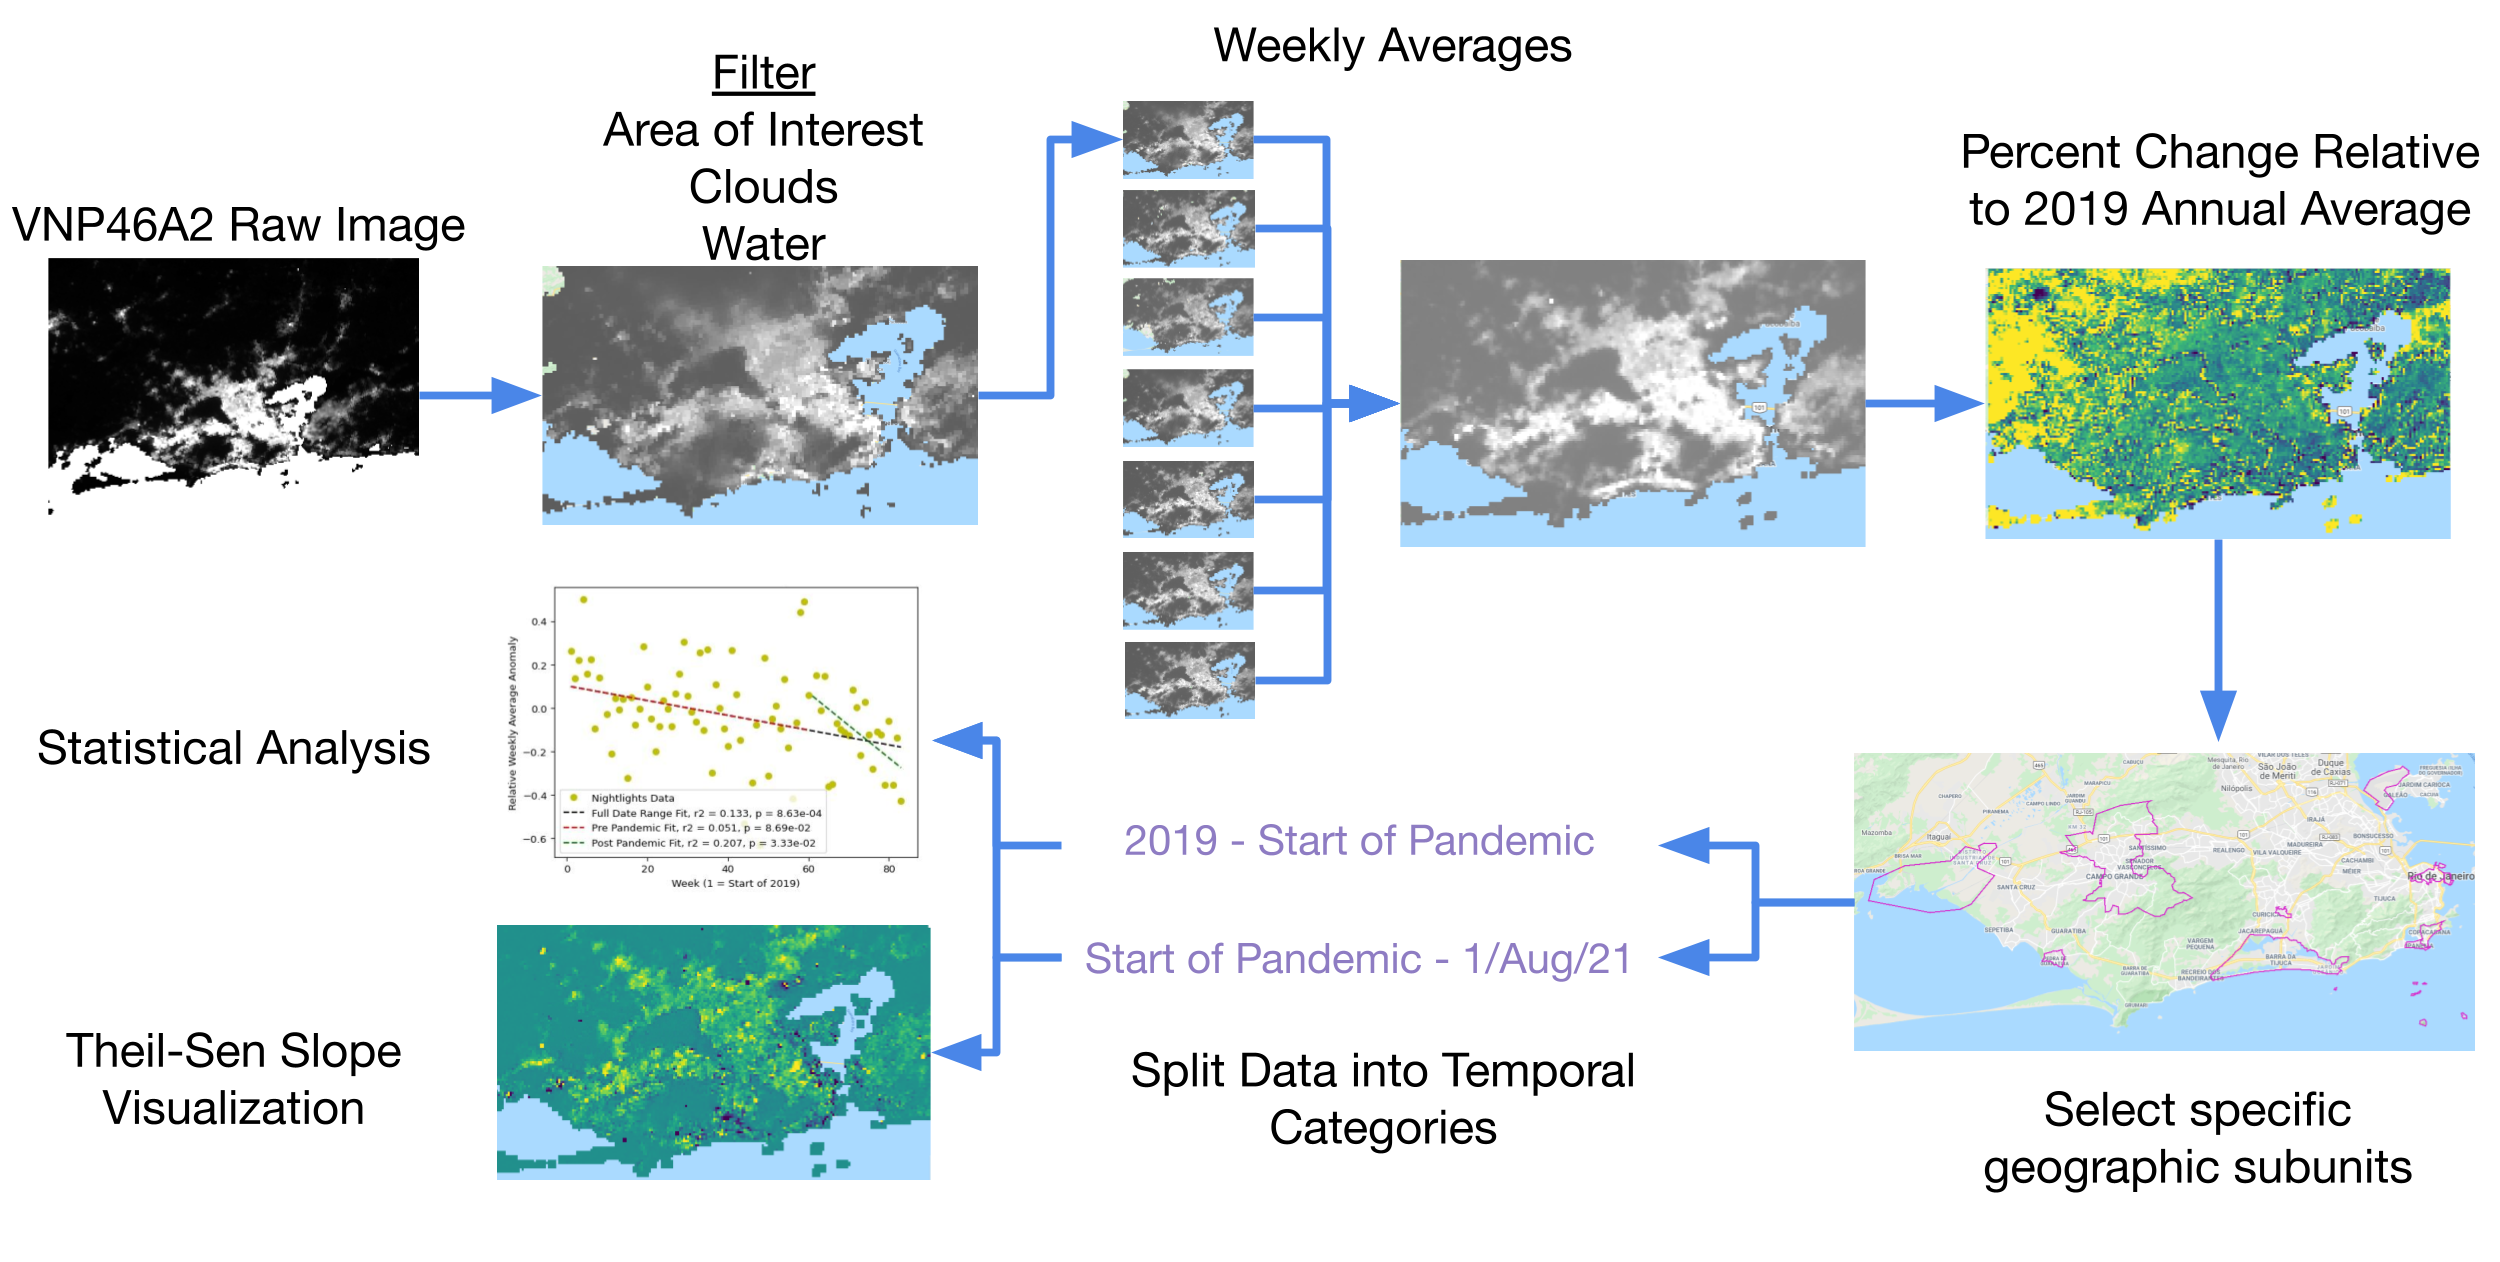
\includegraphics[width=0.9\textwidth]{Figures/chap5/nightlights_method.png}
\caption[Nightlights Processing Methodology]{Method for processing and analyzing nightlight data}
\label{fig:nightlights_method}
\end{figure}


%Data on ship activity can be generated through the use of Sentinel radar imagery by masking out land and permanent structures, then looking for transient bright spots on navigable bodies of water, particularly around major ports. This process can be seen in Figure \ref{fig:ships}. The period of 2018 through the start of the pandemic was used to establish a baseline of ship presence. This was then compared with activity after the onset of the pandemic to identify changes. 
%
%\begin{figure}[!htb]
%	\centering
%	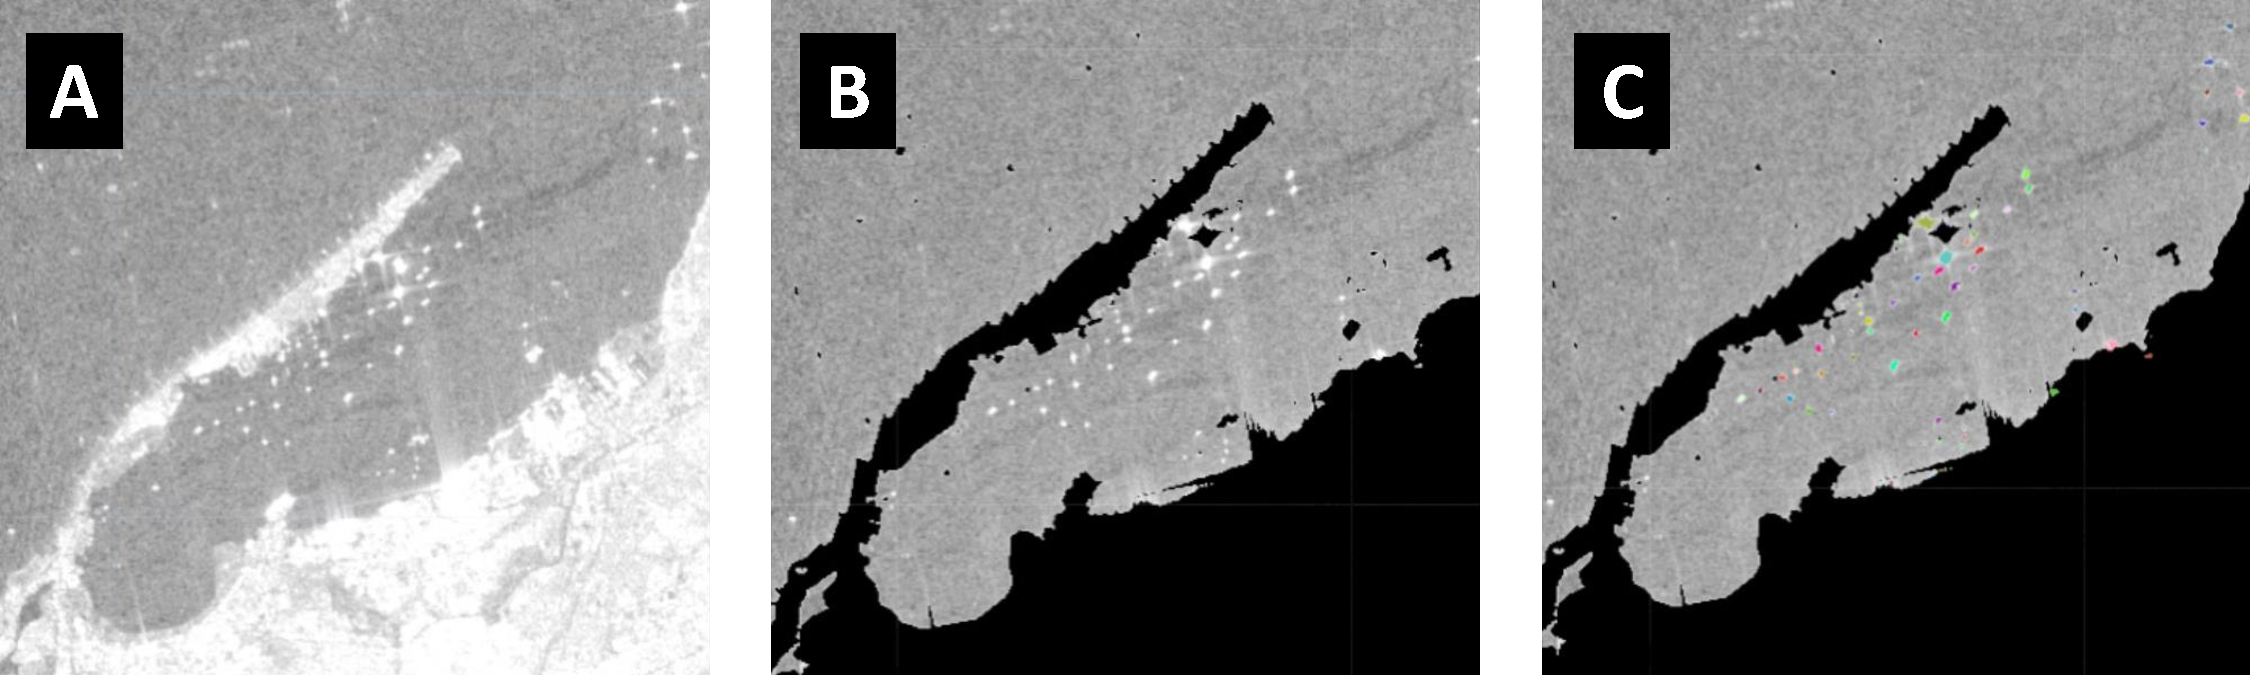
\includegraphics[scale=0.35]{Figures/chap5/ships.pdf}
%	\caption[Ships identification process]{Ships identification process. A: Sentinel-1 SAR imagery of the Luanda area. B: Masking out land and permanent structures. C: Identifying individual ships. Figure created by Amanda Payton.}
%	\label{fig:ships}
%\end{figure}

Beyond mobility and nightlights, Amanda Payton conducted significant analysis of maritime ship activity pre-and-post pandemic onset in the Luanda region using Sentinel-1 \ac{sar} imagery. This is not discussed at length in this thesis as (a) it was not generalized to the other study areas, and (b) I was not significantly involved in this analysis.

Additionally, I performed some experimentation in assessing changes traffic patterns in Rio de Janerio using \ac{eo} imagery, particularly using Sentinel-1 \ac{sar} and higher resolution optical Planet imagery. Further meetings with stakeholders suggested that this was of limited usefulness, particularly in the other locations. This, coupled with a lack of accessible validation data, resulted in us abandoning such efforts fairly early on.

\subsubsection{Decision-making} \label{sec:vida-evdt-decision-method}

Obviously the primary decision axis is containing the spread of coronavirus and properly treating those who are infected. In practice this tends to express itself as various forms of public area and business closures and restrictions, individual social distancing requirements (such as mask wearing), and medical equipment acquisition and allocation. In Rio de Janeiro, for example, many of these policies have been grouped together into a six phase Resumption Plan that has clear indicator-based conditions for when to advance to the next phase \cite{iplanrioIndicadoresPlanoRetomada2020}, which facilitates visualization and simulation in Vida. Most of the locations of interest have similar qualitative, ordinal policy categories, with varying numbers of steps or details. 

We spent some effort at developing a consistent process for transforming such policies from qualitative ordinal categories into quantitative scores, building upon such projects as the CoronaNet Research Project \cite{CoronaNetResearchProject}. This was done both to enable consistent visualizations where various quantitative metrics (active coronavirus cases, air quality, mobility indices, etc.) can be directly compared to policy actions over time (e.g. in Fig \ref{fig:mobility-graphs-rio-santiago}). It also would enable some level of comparison across locations of interest in order to help draw causal relationships and identify the impacts, both positive and negative, of certain policies. Our initial approach to this was to break policies into six different categories:

\begin{enumerate}[itemsep=0pt,parsep=0pt]
\item{Mask Mandates}
\item{Travel Restrictions}
\item{Business and Public Space Closures}
\item{Gathering Restrictions}
\item{Curfews}
\item{School Closures}
\end{enumerate}

For each policy regime, each of these six aspects would be scored on a 1 (highly restrictive) to 10 (no requirements or restrictions) scale. An evenly weighted average was then calculated and then sorted into bins: Strict (average score of less than 3), Significant (at least 3 and less than 5), Moderate (at least 5 and less than 7), Light (at least 7 and less than 9), and Minimal (9 or greater). Ultimately this scoring system was deemed too subjective, so an effort was made to better define specific ranks within such category (e.g. no outdoor events with greater than 15 people vs no outdoor events with greater than 50 people). The local teams for each location of interest were involved in both the definition of these ranks and the categorization of local policies into them. This categorization system is presented in Table \ref{tab:policy-system}. The intent was to develop a weighted average of the 0 to 3 policy strictness scores, with weights based on the importance of that particular policy aspect to \ac{covid} control. Ultimately the Vida project concluded prior to this second round being completed, but I will present what was completed on this front.

These policy timelines were then compared with the telecoms-based mobility data collected as part of the Vulnerability component. These were used to assess both the impact and the duration that various policy changes had on mobility.

\begin{landscape}
\scriptsize

\begin{longtable}{| C{2cm} |  C{2cm} |C{3cm} |C{3cm} |C{3cm} |C{3cm}|}
\caption[COVID-19 Policy Categorization System]{The second version of the \ac{covid} policy categorization system developed as part of the Vida project.}
\label{tab:policy-system} \\ \cline{3-6}
\multicolumn{2}{C{4cm}|}{} & \multicolumn{4}{|C{12cm}|}{\textbf{Policy Strictness}} \\ \hline 
\textbf{Policy Group} & \textbf{Policy} & \textbf{0} & \textbf{1} & \textbf{2} & \textbf{3} \\ \midrule \endfirsthead


\cline{3-6} \multicolumn{2}{C{4cm}|}{} & \multicolumn{4}{|C{12cm}|}{\textbf{Policy Strictness}} \\ \hline

\textbf{Policy Group} & \textbf{Policy} & \textbf{0} & \textbf{1} & \textbf{2} & \textbf{3} \\ \midrule \endhead

\multirow{3}{*}{\rotatebox[origin=c]{90}{\parbox{3.5cm}{\centering\textbf{Restriction \& Regulation of Government Services}}}} & \textbf{Public Recreational Areas} & No closures or restrictions & Public recreational areas are open with some social distancing requirements & 	Public recreational areas have significant capacity limits and/or are only open during certain times & Public recreational areas are largely closed \\ \cline{2-6}

& \textbf{School Closures} & No school closures or restrictions & Large, school-related gatherings/activities prohibited & Most schools are required to operate primarily in a hybrid mode (mix of in person and remote) & Most schools are either closed or operating remotely \\ \cline{2-6}

& \textbf{Public Transit} & No restrictions on public transit & Public transit operational with social distancing and/or hygiene restrictions	 & Public transit operational with <50\% capacity & Public transit closed \\ \hline


\multirow{3}{*}{\rotatebox[origin=c]{90}{\parbox{2.5cm}{\centering\textbf{Travel \& Border Restrictions}}}} & \textbf{Quarantine of Travelers} &  No quarantines required & Self-quarantine encouraged but not enforced & Self-quarantine mandated and enforced & Quarantine in government-managed facilities required \\ \cline{2-6}

& \textbf{International Travel} & No border restrictions & International travel to/from high risk areas is discouraged & International travel to/from high risk areas is largely prohibited & International travel is largely prohibited \\ \cline{2-6}

& \textbf{International Shipping} & No border restrictions & Restrictions or precautions taken with commercial traffic from high risk areas & Restrictions or precautions taken with commercial traffic from most or all locations & International traffic heavily restricted from most or all locations \\ \noalign{\penalty-100000} \hline


\multirow{3}{*}{\rotatebox[origin=c]{90}{\parbox{3.5cm}{\centering\textbf{Social Distancing}}}} & \textbf{Stay-at-Home-Orders} & No lockdown & Long distance domestic travel restricted & Specific activities and visits to specific places allowed, other activities restricted & Specific activities and visits to specific places allowed and are confined to specific hours, other activities restricted \\* \cline{2-6}

& \textbf{Masks} & No mask requirements & Masks wearing in public spaces is encouraged but not required & Masks required to be worn in indoor public spaces but not outdoors & Masks required to be worn in both indoor and outdoor public spaces \\* \cline{2-6}

& \textbf{Mass Gatherings} & No restrictions on mass gatherings & Indoor gatherings of >50 prohibited, little or no restrictions on outdoor gatherings & Most or all indoor gatherings prohibited, outdoor gatherings of >100 prohibited & Most or all mass gatherings, indoor or outdoor, are prohibited \\* \hline



\multirow{2}{*}{\rotatebox[origin=c]{90}{\parbox{2cm}{\centering\textbf{Restriction and Regulation of Businesses}}}} & \textbf{Essential Businesses} & No closures or restrictions & Most or all essential businesses are open, but must take social distancing measures & Most or all essential businesses must operate with <50\% capacity & Most or all essential businesses must operate via curbside pickup or delivery \\* \cline{2-6}

& \textbf{Non-essential Businesses} & No closures or restrictions & Most or all non-essential businesses are open, but must take social distancing measures & Most or all non-essential businesses must operate with <50\% capacity & Most or all non-essential businesses are closed \\ \bottomrule



\end{longtable}
\end{landscape}



%\begin{landscape}
%\begin{table}[!htb]
%\caption[COVID-19 Policy Categorization System]{The second version of the \ac{covid} policy categorization system developed as part of the Vida project.}
%\label{tab:policy-system}
%\begin{center}
%\tiny
%\begin{tabular}{| C{1cm} |  C{1.75cm} |C{1.75cm} |C{1.75cm} |C{1.75cm} |C{1.75cm} |C{1.75cm} |C{1.75cm} |C{1.75cm} |C{1.75cm} |C{1.75cm} |C{1.75cm} |} \hline
%
%& \multicolumn{2}{|C{3.5cm}|}{\textbf{Restriction \& Regulation of Government Services}} & \multicolumn{3}{|C{5.25cm}|}{\textbf{Travel \& Border Restrictions}} & \textbf{Lockdown} & \multicolumn{3}{|C{5.25cm}|}{\textbf{Social Distancing}} &  \multicolumn{2}{|C{3.5cm}|}{\textbf{Restriction \& Regulation of Business}} \\ \hline
% 
%\textbf{Strictness} & \textbf{Public Recreational Areas} & \textbf{School Closures} & \textbf{Quarantine of Travelers} & \textbf{International Travel} & \textbf{International Shipping} & \textbf{Stay-at-Home Orders} & \textbf{Masks} & \textbf{Public Transit} & \textbf{Mass Gatherings} & \textbf{Essential Businesses} & \textbf{Non-Essential Businesses} \\ \hline
% 
%0 & No closures or restrictions & No school closures or restrictions & No quarantines required & No border restrictions & No border restrictions	& No lockdown & No mask requirements	& No restrictions on public transit	& No restrictions on mass gatherings	& No closures or restrictions & No closures or restrictions \\ \hline 
%
%1 & Public recreational areas are open with some social distancing requirements & Large, school-related gatherings/activities prohibited & Self-quarantine encouraged but not enforced & International travel to/from high risk areas is discouraged & Restrictions or precautions taken with commercial traffic from high risk areas & Long distance domestic travel restricted & Masks wearing in public spaces is encouraged but not required & Public transit operational with social distancing and/or hygiene restrictions & Indoor gatherings of >50 prohibited, little or no restrictions on outdoor gatherings & Most or all essential businesses are open, but must take social distancing measures & Most or all non-essential businesses are open, but must take social distancing measures \\ \hline
%
%2 & Public recreational areas have significant capacity limits and/or are only open during certain times & Most schools are required to operate primarily in a hybrid mode (mix of in person and remote) & Self-quarantine mandated and enforced & International travel to/from high risk areas is largely prohibited & Restrictions or precautions taken with commercial traffic from most or all locations & Specific activities and visits to specific places allowed, other activities restricted & Masks required to be worn in indoor public spaces but not outdoors & Public transit operational with <50\% capacity & Most or all indoor gatherings prohibited, outdoor gatherings of >100 prohibited & Most or all essential businesses must operate with <50\% capacity & Most or all non-essential businesses must operate with <50\% capacity \\ \hline
%
%3 & Public recreational areas are largely closed & Most schools are either closed or operating remotely & Quarantine in government managed facilities required & International travel is largely prohibited & International traffic heavily restricted from most or all locations & Specific activities and visits to specific places allowed and are confined to specific hours, other activities restricted & Masks required to be worn in both indoor and outdoor public spaces & Public transit closed & Most or all mass gatherings, indoor or outdoor, are prohibited & Most or all essential businesses must operate via curbside pickup or delivery & Most or all non-essential businesses are closed \\ \hline
%
%
%\end{tabular}
%\end{center}
%\end{table}
%
%\end{landscape}




\subsubsection{Technology}

Various forms of sensing technology are relevant during a viral epidemic. While our team was primarily focused on satellite-based earth observation technology and in-situ environmental sensors, another key form of relevant sensing technology is coronavirus testing (both the technology of the individual tests and the social technology that is the regional testing regime). Rates of \ac{pcr} testing can be integrated into the public health model through its influence on the difference (or lack thereof) and delay between the estimated number of active infections and the measured infections. Similarly to Chapter \ref{ch:mangroves}, the technology design and selection capabilities of the \ac{evdt} Framework were largely not explored in this case study. 

\subsection{EVDT Results} \label{sec:vida-evdt-result}

\subsubsection{Environment} \label{sec:vida-evdt-e-result}

For each bairro in Rio de Janeiro, calculated weekly median PM10 levels, calculated a seasonal sinusoidal correction, and a linear secular correction. Figure \ref{fig:aq-combined} shows this process for the Centro bairro. We then ran two-samples t-tests and Anderson Darling tests on the normalized histograms of the pre-and-post pandemic variation-corrected PM10 data, assuming that the pre-pandemic distribution was approximately normally distributed. These tests determine if the pre-pandemic and post-pandemic PM10 measurements are actually different. In particular, as seen in Figure \ref{fig:pm}, we found that tourist areas had a significant decrease in measured PM10 post-pandemic, while some rural or residential areas had slight decreases. We found a significant increase in PM10 measurements post-pandemic in the downtown/business district, with some smaller increases in mixed use/residential and recreational areas. 

\clearpage

\begin{figure}[H]
\centering
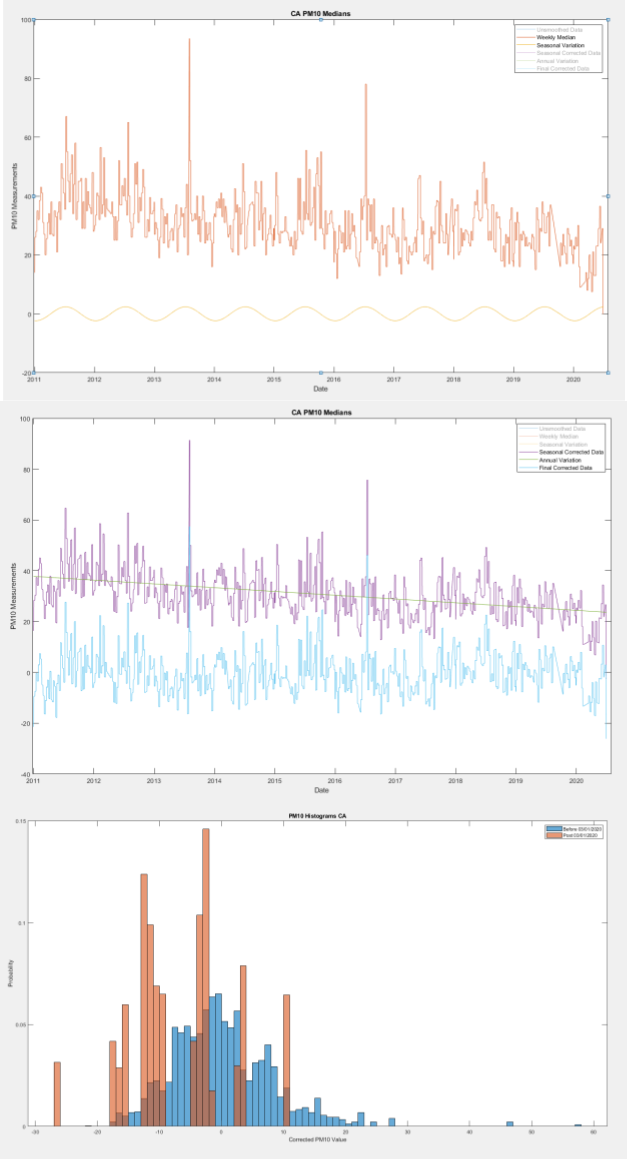
\includegraphics[width=0.6\textwidth]{Figures/chap5/aq-combined.png}
\caption[PM10 Normalization for the Centro bairro of Rio de Janeiro]{Normalization results for PM10 in the Centro bairro of Rio de Janeiro. Top: A sinusoidal correction for seasonal variation. Middle: A linear correction for secular variation. Bottom: Comparison of the corrected pre-and-post pandemic PM10 distributions.}
\label{fig:aq-combined}
\end{figure}


\begin{figure}[!htb]
\centering
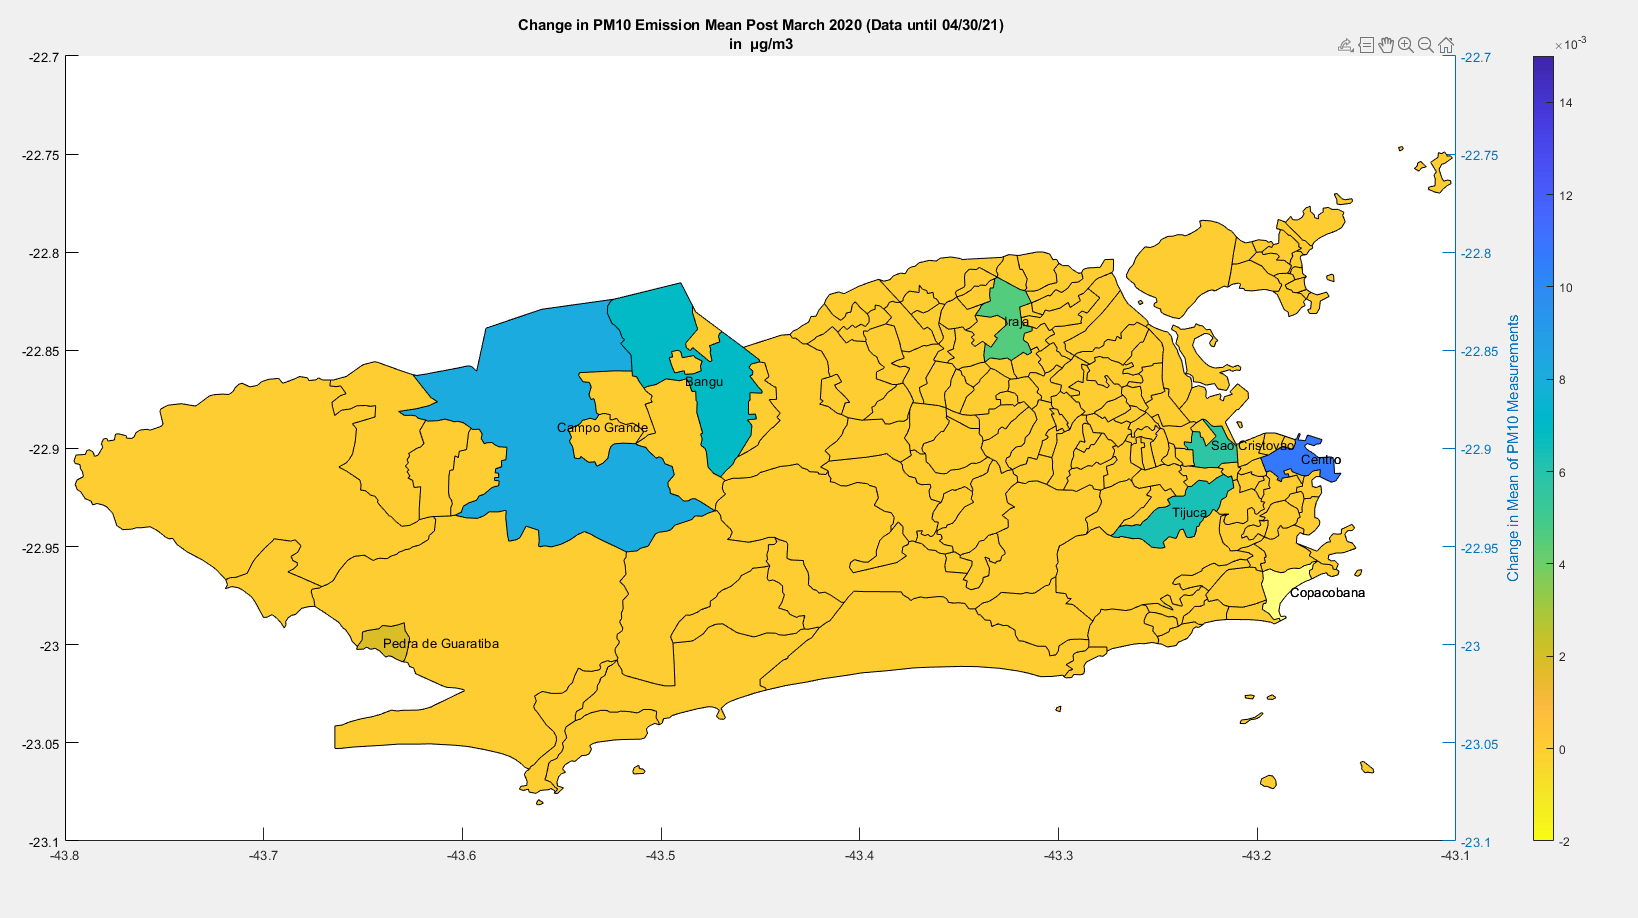
\includegraphics[width=0.9\textwidth]{Figures/chap5/pm10.png}
\caption[Changes in PM10 in Rio de Janeiro]{Changes in PM10 levels in several bairros of Rio de Janeiro during the first two months of the pandemic, normalized for intraweek, seasonal, and annual trends.}
\label{fig:pm}
\end{figure}

\subsubsection{Public Health}

The simulation-related results are presented in Section \ref{sec:vida-dss} as part of the presentation on the Vida \ac{dss}. Here I will focus on briefly describing the historical data for the first year of the pandemic. The confirmed per-capita \ac{covid} cases for this period are shown in Figure \ref{fig:combined-cases}. 

Several aspects immediately jump out. First, is that the magnitudes of the cases very immensely across locations with Indonesia, Querétaro and Angola having much lower cases per-capita than Rio de Janeiro or Metropolitana. This can be attributed to a few different causes. First are the different geographic scales that each of these datasets represent. It is no coincidence that the two areas representing dense metropolitan areas have the higher recorded cases and the areas representing larger geographic areas (including much less densely populated areas) have much lower. Population density affects the spread and intensity of the spread of \ac{covid}. This is also linked to another potential cause of the difference in recorded cases: testing regimes. The dense metropolitan areas likely had much more systematic testing regimes in place, resulting in a higher portion of total \ac{covid} cases being recorded (and made a part of these statistics). This phenomena lead to the Ministerio de Salud, el Ministerio de Ciencias commissioning an estimate of the total number of \ac{covid} cases (including those unrecorded by tests) \cite{icovidDatosCOVID19OutputProducto532020}. It also led to the differentiation of the \textit{Measured Infected Population} and the actual infected population in the \ac{sir} model in Figure \ref{fig:vida_sd}.

Another aspect worth pointing out is first evidence of multiple waves of cases, most notable in the Rio de Janeiro curve. This was a common phenomena around the world over the course of the subsequent years and was noted as an important phenomena to capture in the \ac{sir} model to be used in the \ac{dss}. 

\begin{figure}[!htb]
\centering
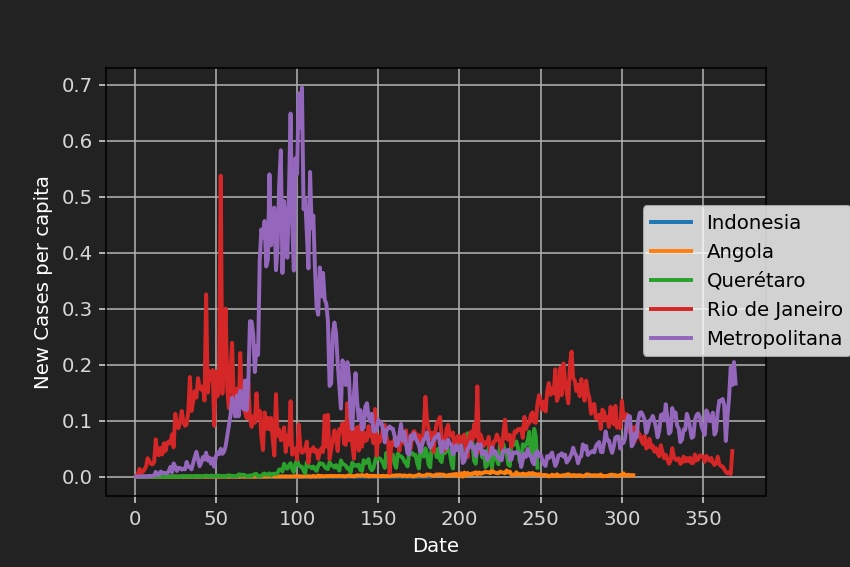
\includegraphics[width=0.7\textwidth]{Figures/chap5/combined-cases.jpg}
\caption[COVID-19 Cases Over Time]{Recorded per-capita \ac{covid} cases approximately the first year of the pandemic in each of the study locations.}
\label{fig:combined-cases}
\end{figure}

\subsubsection{Vulnerability} \label{sec:vida-evdt-v-result}

\paragraph{Telecommunications Mobility} \leavevmode\newline

Telecoms-based mobility data proved to be a powerful way of understanding how the populations of the study areas were responding to changes in both \ac{covid} case loads and official response policies. The relationship with the latter is explored more in Section \ref{sec:vida-evdt-decision-results} but here it is worth noting some important phenomena in the mobility data itself.

Figure \ref{fig:transit-mobility-comparison} shows the transit-related mobility index from Google's \ac{covid} Community Mobility Reports for each of the study areas \cite{googleCOVID19CommunityMobility}, along with several notable phenomena across the locations. While the following section will explore the study areas more individually, the overall trend across the locations is remarkably similar. 

\begin{figure}[!htb]
\centering
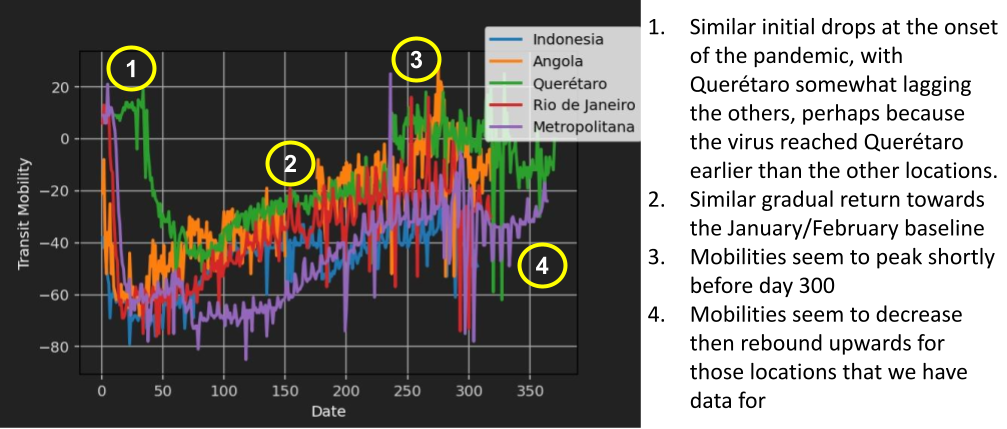
\includegraphics[width=0.9\textwidth]{Figures/chap5/transit-mobility-comparison.png}
\caption[Transit Mobility Over Time for All Locations]{Comparison of the transit mobility index across each of the locations over time.}
\label{fig:transit-mobility-comparison}
\end{figure}

Not all forms of mobility showed this general trend of a sudden decrease followed by a long climb. As might be expected, the residential mobility index moved in the opposite direction as individuals suddenly found themselves spending much more time at home during the initial months of the pandemic. This is shown for Angola in Figure \ref{fig:policy-residential-mob}.

\begin{figure}[!htb]
\centering
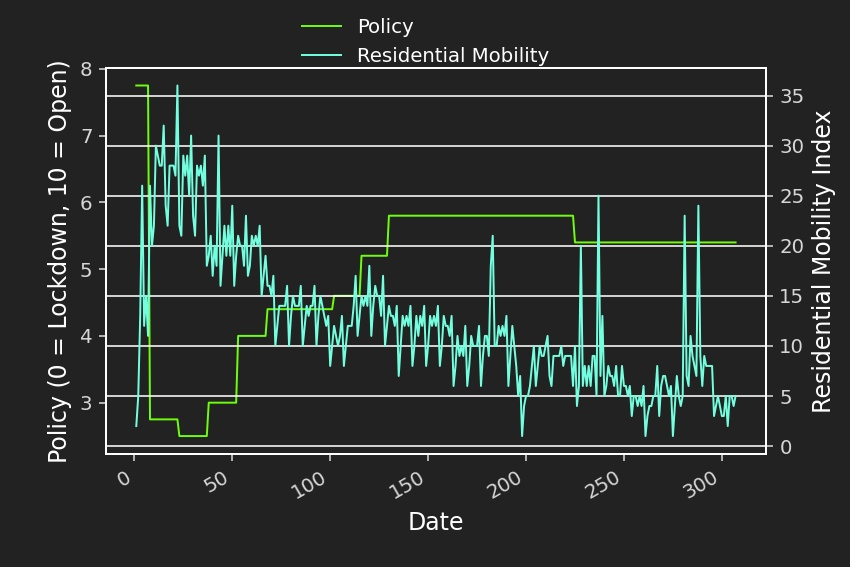
\includegraphics[width=0.7\textwidth]{Figures/chap5/Policy_nat_residential_mob.jpg}
\caption[Angola COVID-19 Policy \& Residential Mobility]{Comparison of the Angola \ac{covid} response policy strictness and the residential mobility index over time.}
\label{fig:policy-residential-mob}
\end{figure}

\paragraph{Urban Nightlights} \leavevmode\newline

Similarly to other researchers, we detected significant changes in nightlights due to the onset of COVID-19 and later policy changes \cite{elvidgeDimmingLightsChina2020, xbsdScipy2021Predicting2021}. In particular, areas associated with air travel and tourism experienced significant decreases in nightlights and associated human activity (areas in purple along the eastern and southern edges of Rio de Janeiro in Figure \ref{fig:nlts}). Downtown and commercial areas experienced a similar, though less dramatic decrease. Primarily residential areas (the yellow, east-west arc across the middle of Figure \ref{fig:nlts}), meanwhile, significantly brightened. These trends are apparent both for relative percentage change across these areas and when the changes are normalized for long term trends. Graphs showing such changes for airports and specific tourist-centric areas in Rio de Janeiro, Brazil and Bali, Indonesia can be seen in Figure \ref{fig:nlg}. 

The results of basic statistical analysis, particularly t-tests to determine if pre-pandemic and post-pandemic brightness are actually different, for various bairros and areas of Rio de Janeiro can be seen in Figure \ref{fig:nstats}. These results mutually confirm each other and point towards the potential of urban nightlight imagery to supplement telecoms-based mobility data.

\begin{figure}[!htb]
\centering
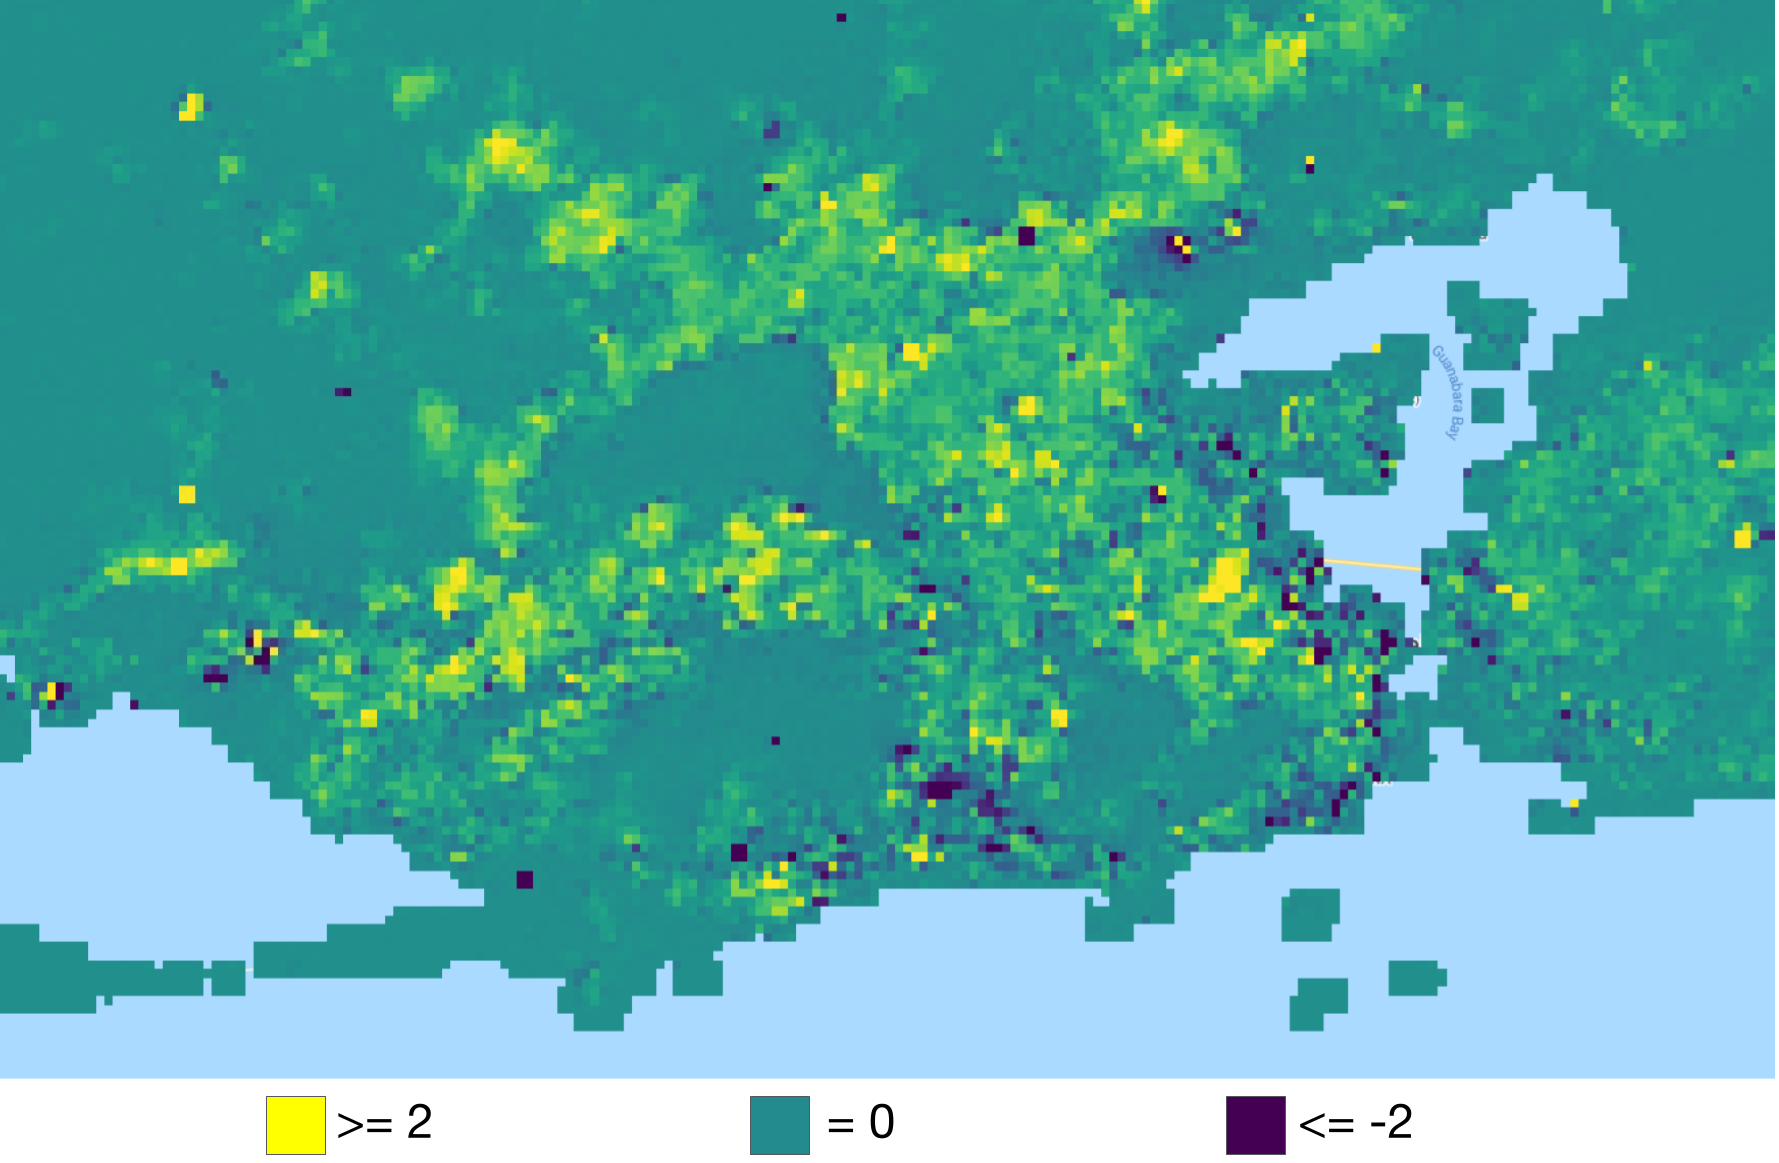
\includegraphics[width=0.9\textwidth]{Figures/chap5/Nightlights_TS.png}
\caption[Changes in nightlights in Rio de Janeiro]{Theil-Sen trend estimator for normalized changes in nightlights in Rio de Janeiro during the initial phases of the pandemic (March 1st to August 30th, 2020).}
\label{fig:nlts}
\end{figure}

\begin{figure}[!htb] 
\centering
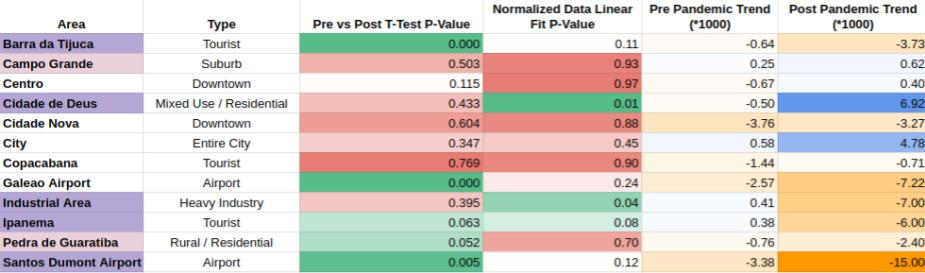
\includegraphics[width=0.9\textwidth]{Figures/chap5/RioNightStats.jpg}
\caption[Nightlight Statistics for Rio de Janeiro]{Statistics for nightlight trends in several bairros (neighborhoods) and areas of Rio de Janeiro. Greens indicate stronger statistical significance, red less. Yellows indicate negative trends, blue positive.}
\label{fig:nstats}
\end{figure}


\clearpage

\begin{figure}[!htb] 
\centering
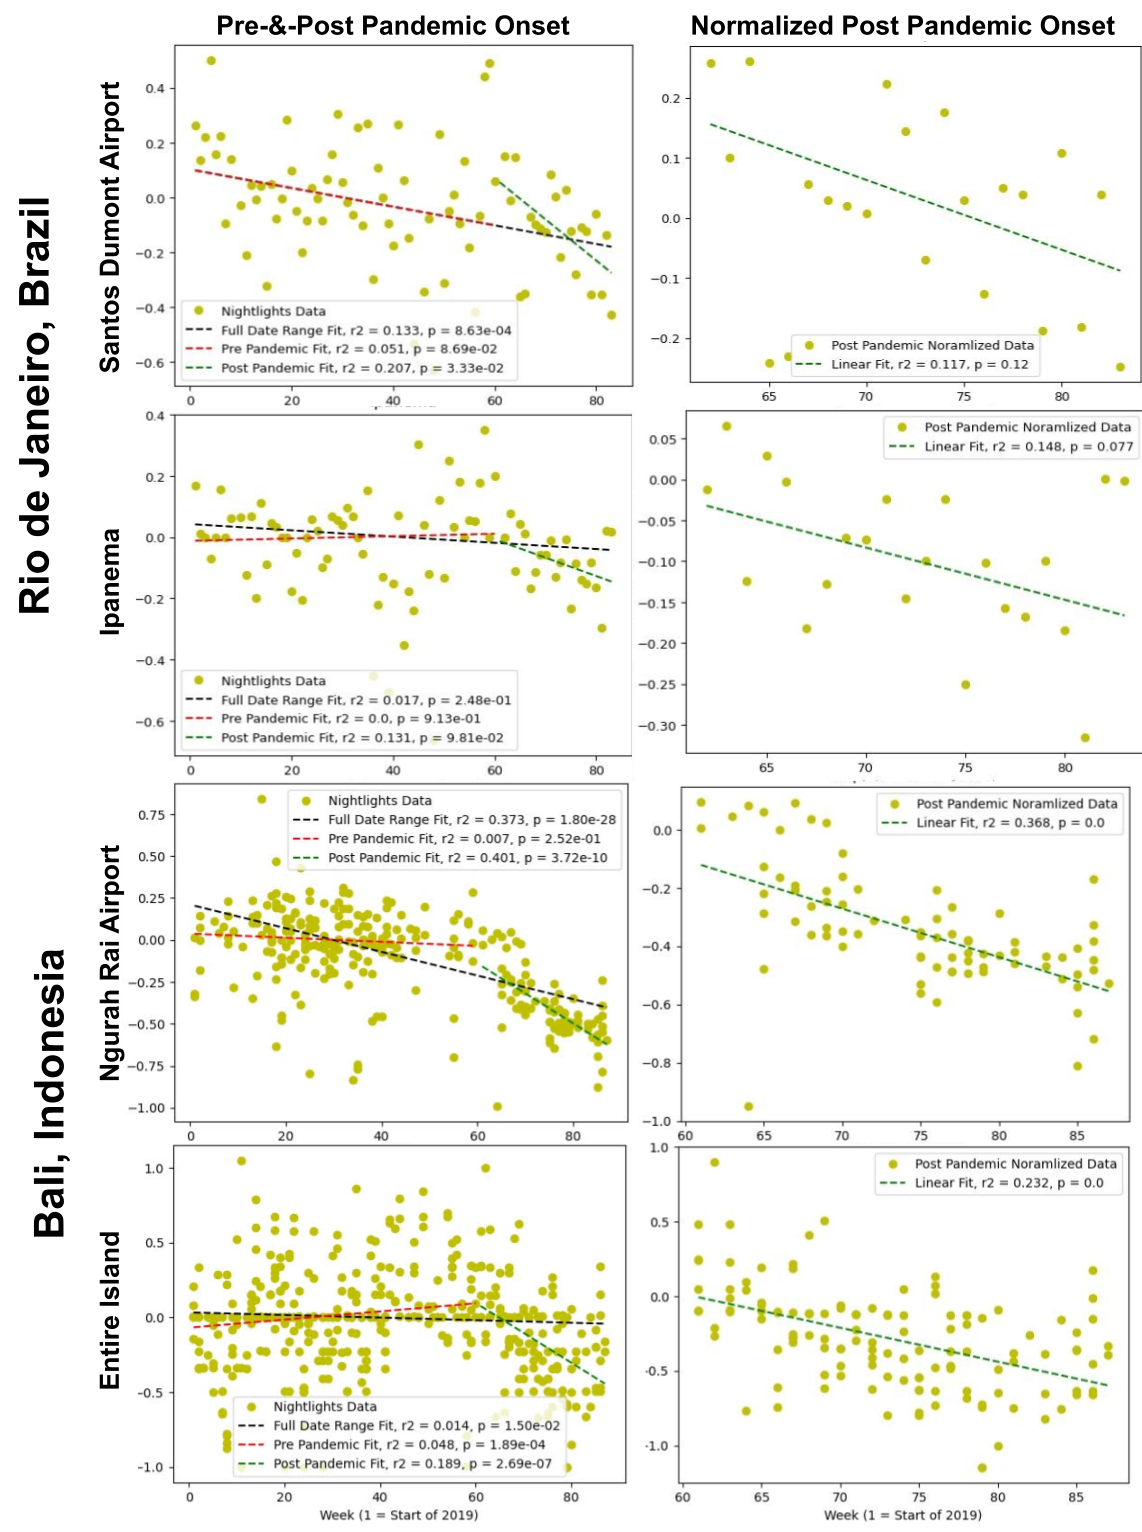
\includegraphics[width=0.85\textwidth]{Figures/chap5/Nightlights_Graphs.png}
\caption[Nightlight Trends for Rio de Janeiro and Bali]{Pre-and-post pandemic nightlight trends for Rio de Janeiro and Bali, showing both airports and tourist-centric areas.}
\label{fig:nlg}
\end{figure}

%\paragraph{Ship Tracking} \leavevmode\newline
%
%Initial results regarding ship tracking in the harbor of Luanda, Angola suggest that there may be a measurable change in ship number and location related to the pandemic. Compared to the preceding two years, the monthly average number of ships within the Bay increased slightly after the onset of the pandemic and continued to remain higher throughout the year. In the offshore area outside of the bay, the average monthly number of ships was lower than in the two years preceding the pandemic. As the number of \ac{covid} cases in the country climbed, the number of ships within the bay further increased, while the number of ships in the offshore area decreased (as shown in Figure \ref{fig:shipst}). The extended docking within the harbor could reflect a reduction in ships conducting trade or delays in the process of loading and unloading ships due to \ac{covid}.  Further investigation is needed into the accuracy and statistical significance of these results in order to draw conclusions. However, at this early stage of analysis it appears that detecting changes in economic proxies such as ship movement using satellite imagery is possible and we plan to extend our analysis to other regions for comparison.
%
%\begin{figure}[!htb]
%\centering
%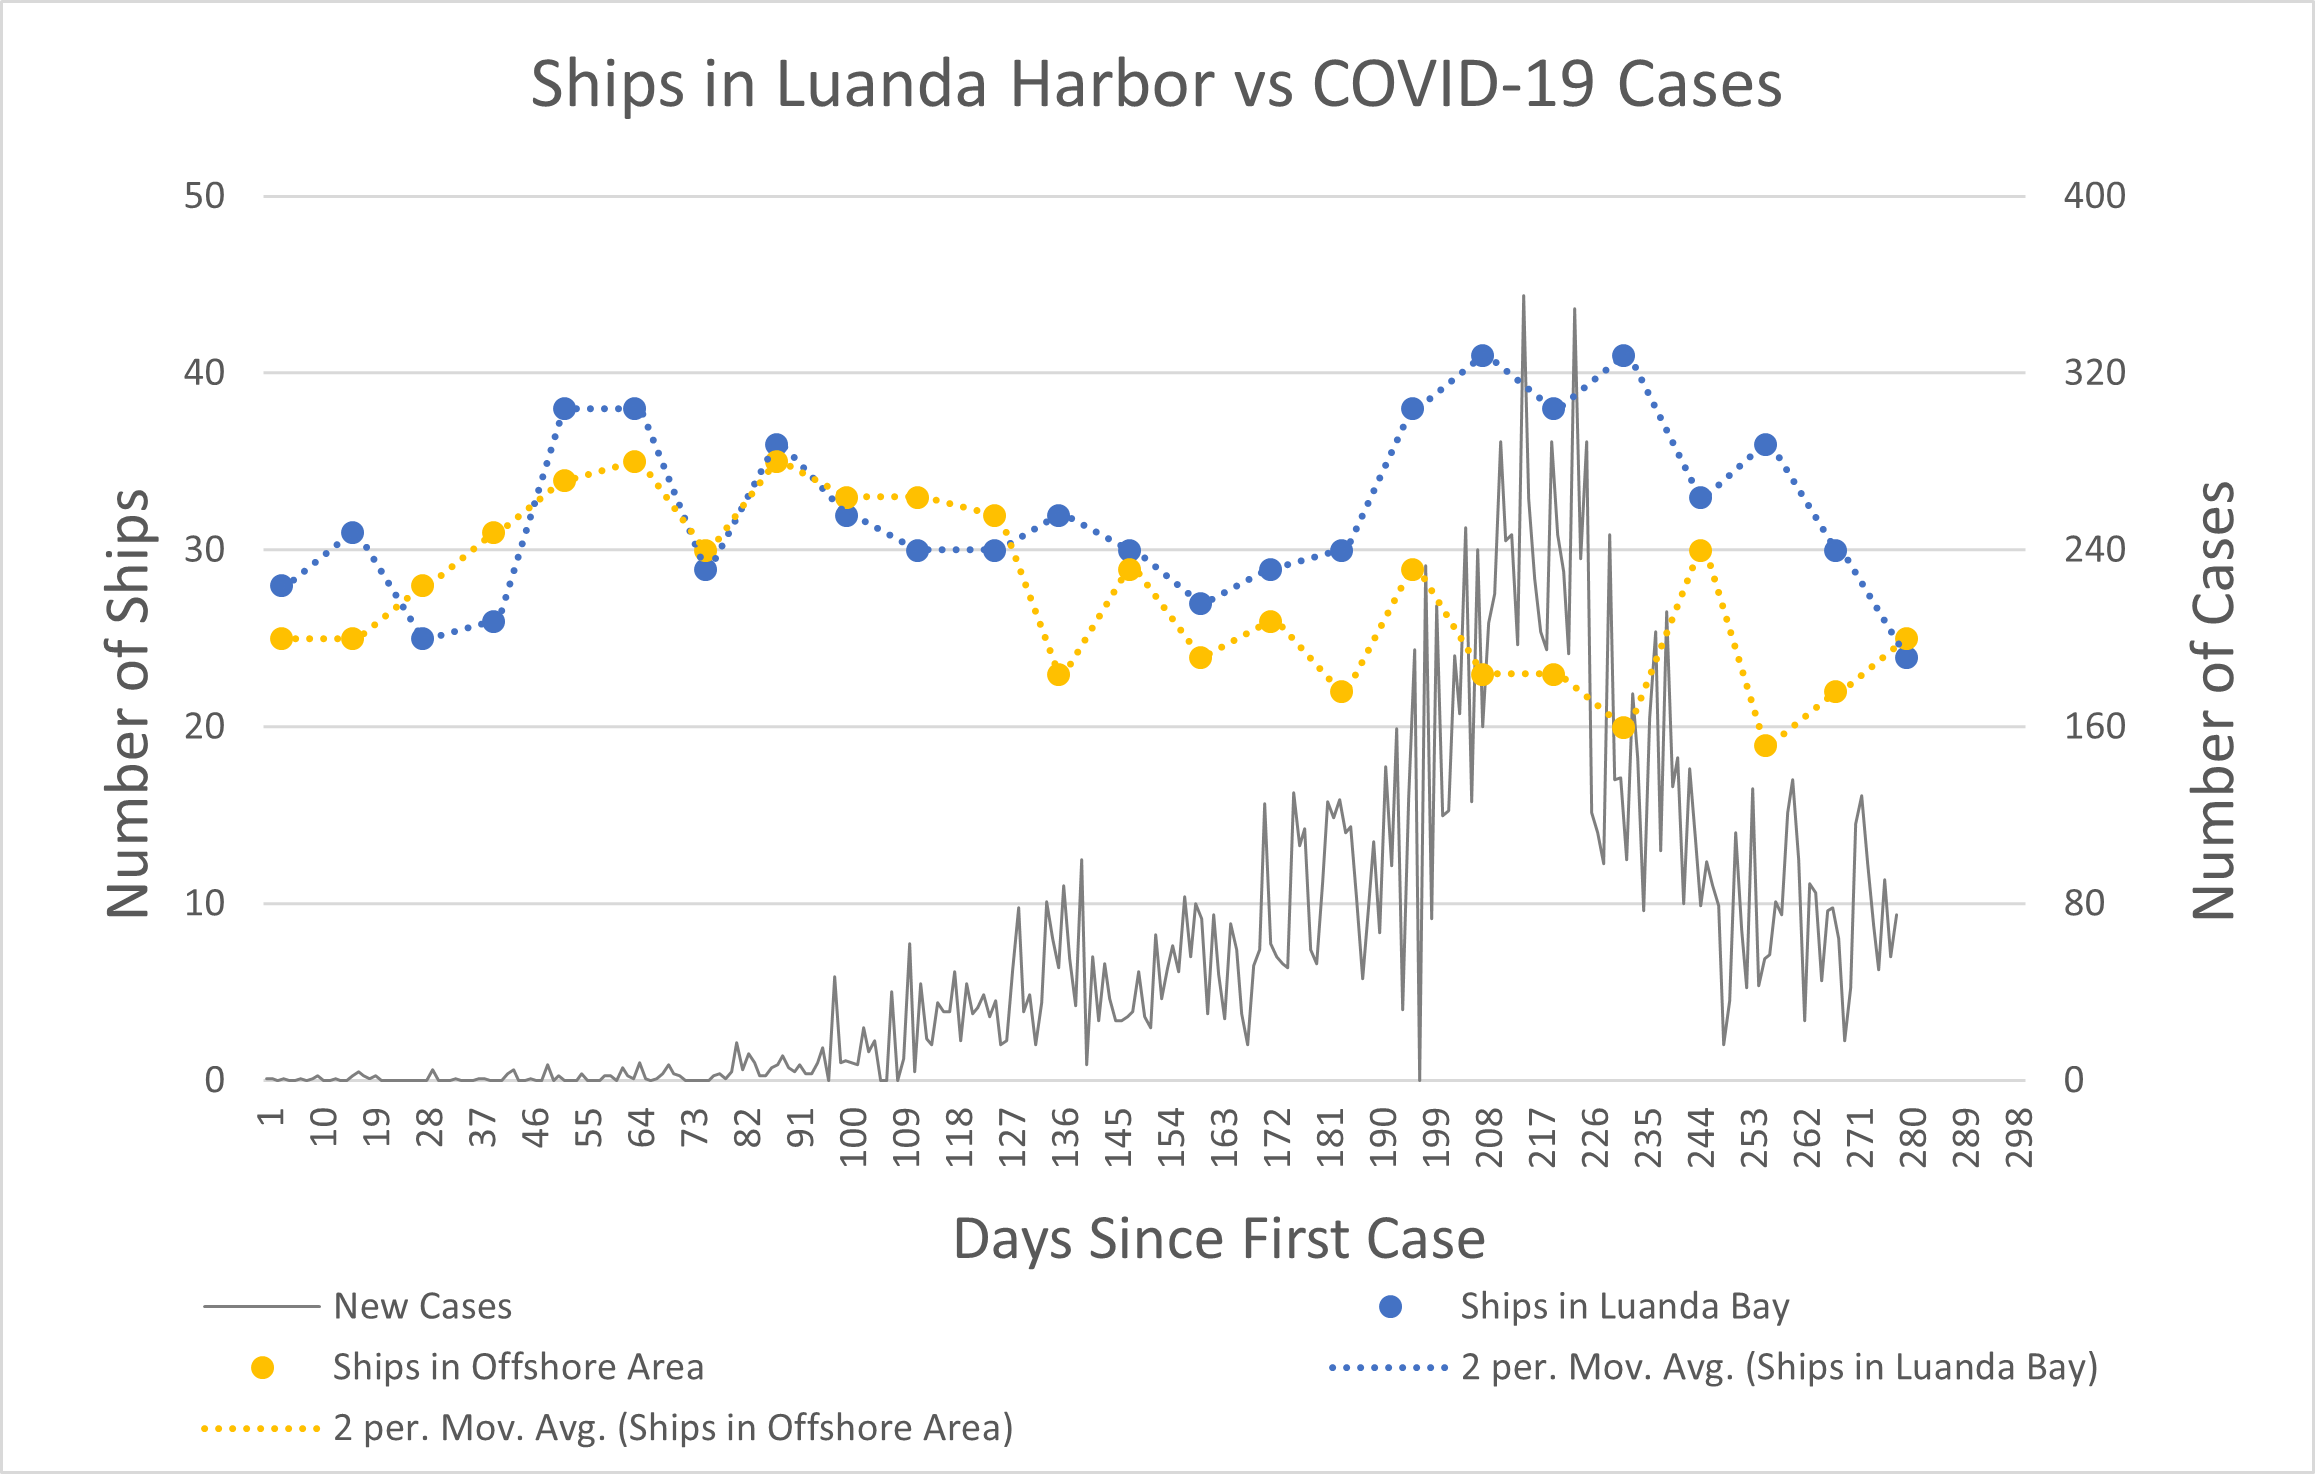
\includegraphics[width=0.9\textwidth]{Figures/chap5/ships_over_time.png}
%\caption{Ship presence over time for the Luanda area.}
%\label{fig:shipst}
%\end{figure}

\subsubsection{Decision-Making} \label{sec:vida-evdt-decision-results}

The initial version of the \ac{covid} response policy quantification/scoring can be seen in Figure \ref{tab:covid-policy-scores}. In this chart, we can see a similar wave of initial closures, all happening within the initial days or weeks of the pandemic, though with varying levels of strictness. After some period of time, every location made some effort to re-open, though the start date of this varied significantly from around Day 80 (Jakarta, Indonesia) to around Day 210 (Metropolitana, Chile). After these initial attempts at re-opening, the locations diverge with some re-implementing stricter policies in response to subsequent waves (Indonesia and Metropolitana) and others seeking to remain on a re-opening trajectory (Querétaro, Angola, and Indonesia).

More details on what each policy regime entailed and how they were scored is provided in Appendix \ref{app:policy-summary}. 

\begin{figure}[!htb]
\centering
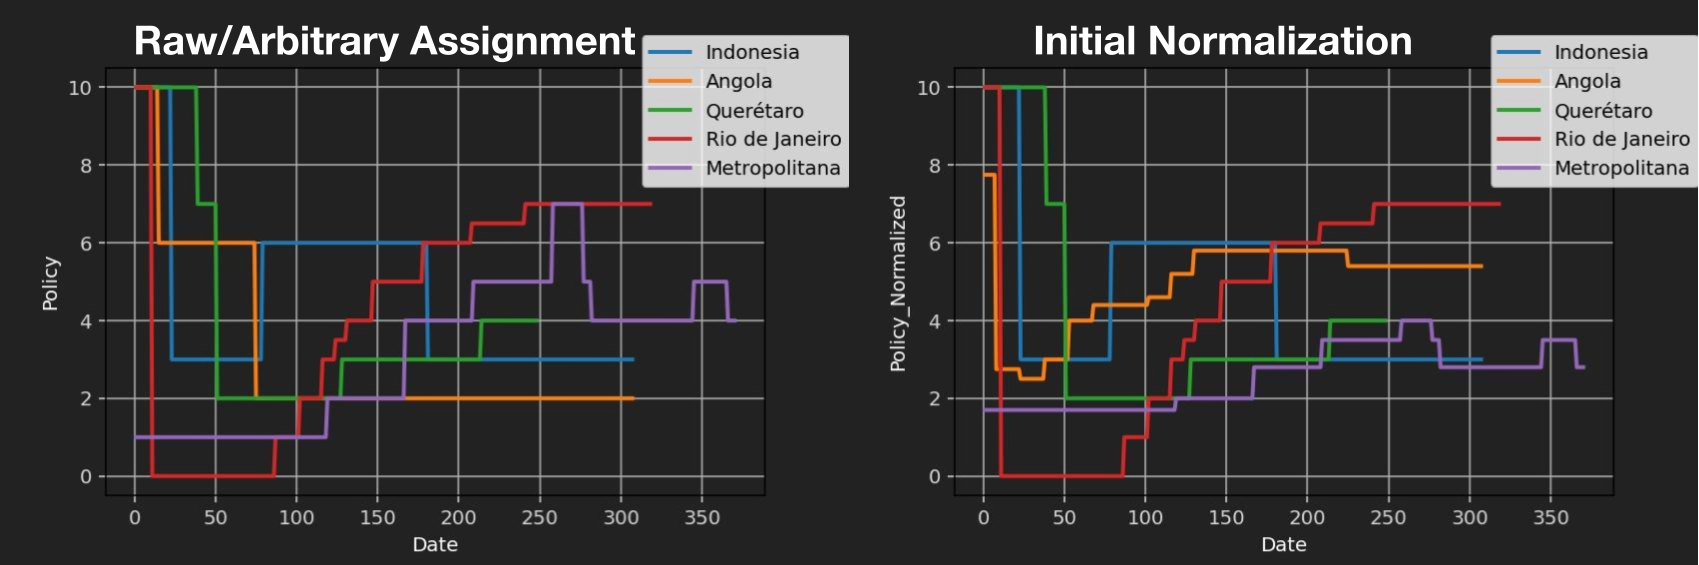
\includegraphics[width=0.9\textwidth]{Figures/chap5/policy-comparison.png}
\caption[COVID-19 Policy Strictness Over Time]{\ac{covid} policy strictness over time for each of the study areas, comparing the original, arbitrary numerical assignments with the initial round of normalization.}
\label{fig:policy-comparison}
\end{figure}

Telecommunications-based measurements of Vida have also provided insightful for decision-makers. Figures \ref{fig:mobility-graphs-rio-santiago} and \ref{fig:mobility-graphs-angola-jakarta} compare mobility with active coronavirus cases and policy status across each of the study locations, noting particular notable phenomena. Some variations are unsurprising: a upward spike during Chile's constitutional referendum, downward spikes for the winter holidays. Others are more relevant for policy-making. Specifically, once the number of active cases declines, mobility increases even if policies remain restrictive. This suggests that the population's perception of infection risk (subject to growing desensitization) may have a stronger impact on mobility than official policy, at least during re-opening.

\clearpage

\begin{figure}[!htb]
\centering
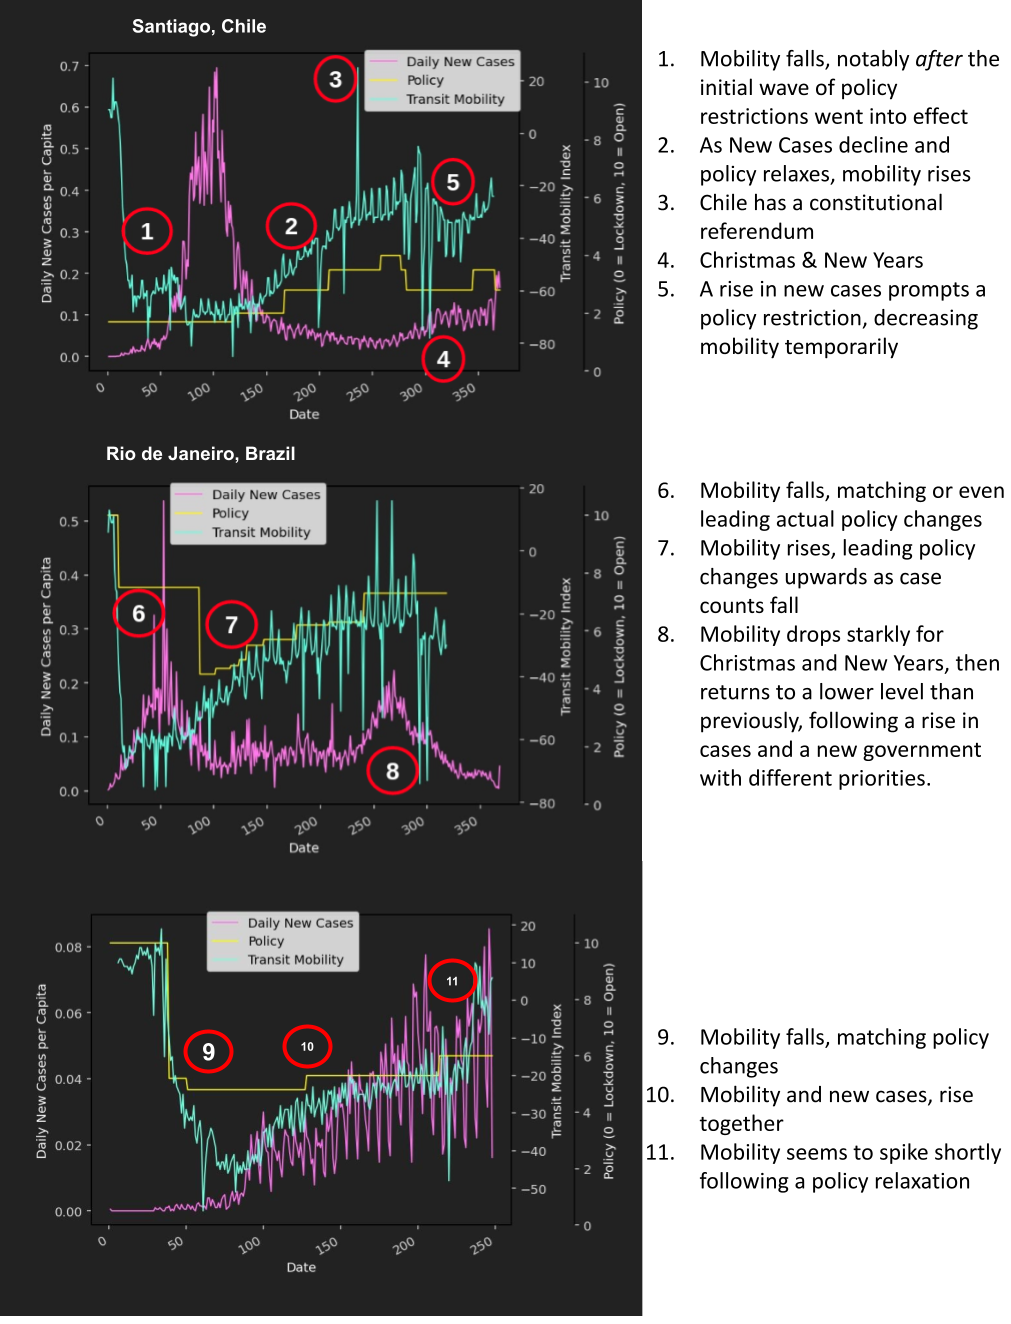
\includegraphics[width=0.8\textwidth]{Figures/chap5/mobility-graphs-rio-santiago.png}
\caption[Mobility, COVID, \& policy in Rio de Janeiro, Santiago, and Querétaro]{Comparisons of coronavirus cases, policy changes, and mobility for Rio de Janeiro, Santiago, and Querétaro.}
\label{fig:mobility-graphs-rio-santiago}
\end{figure}

\begin{figure}[!htb]
\centering
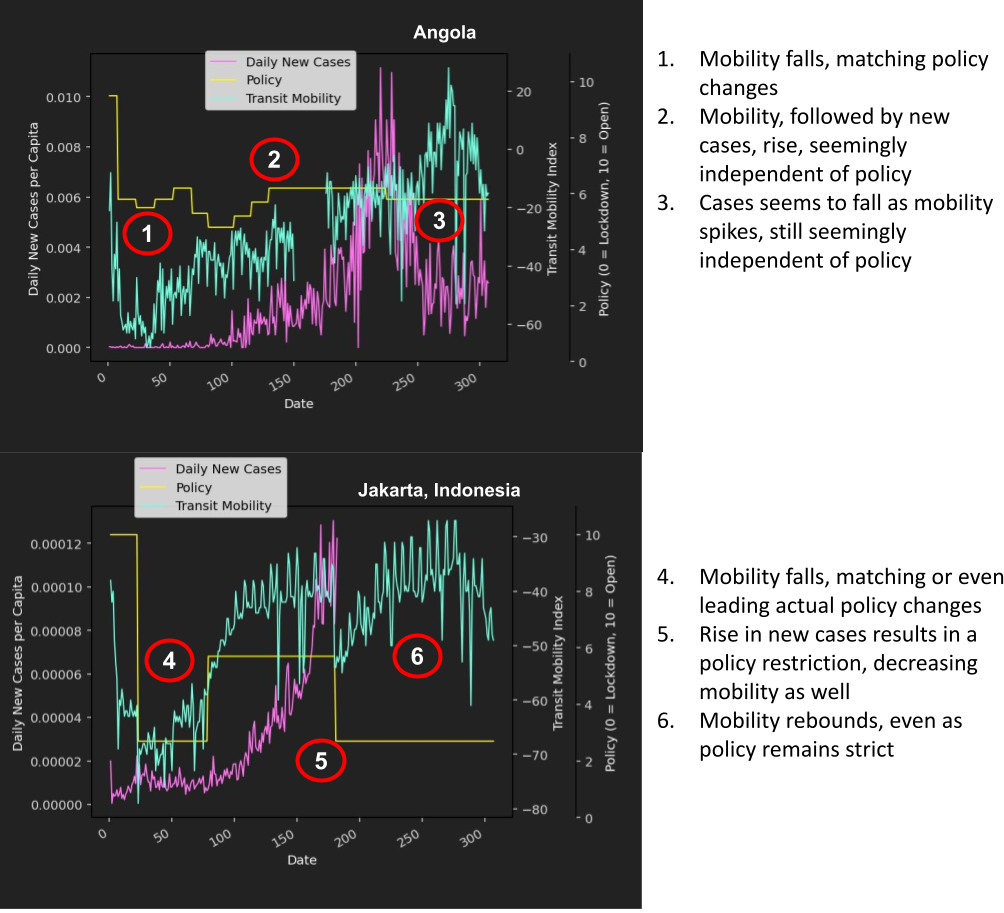
\includegraphics[width=0.8\textwidth]{Figures/chap5/mobility-graphs-angola-jakarta.png}
\caption[Mobility, COVID, \& policy in Angola and Jakarta]{Comparisons of coronavirus cases, policy changes, and mobility for Angola and Jakarta.}
\label{fig:mobility-graphs-angola-jakarta}
\end{figure}

\subsubsection{Technology}

Over the past several sections we saw significant differences in data availability across the study locations, with resulting differences in scale and comparability, as particularly noted in the Public Health component. This was exacerbated by the fact that the issues of highest priority to stakeholders (namely \ac{covid} cases and response policies) were not directly measurable by remote observation. The future possibility of using the \ac{evdt} Framework for designing testing regimes is discussed further in Section \ref{sec:vida-discuss}.


\section{Decision Support System} \label{sec:vida-dss}

The lessons, data, and analysis from the \ac{saf} (Section \ref{sec:vida-saf}) and the \ac{evdt} framing (Section \ref{sec:vida-evdt}) were used to design and develop a \acf{dss}. To revisit the System Functions, the primary functions of the \ac{dss} were to:

\begin{itemize}[itemsep=0pt,parsep=0pt]
	\item{\textbf{Visualize historical public health data and other relevant data.} The public health data includes \ac{covid} cases, deaths, and hospitalizations, among others. The relevant non-public-health data is based on the priorities of each study area but include such things as \ac{covid} response policy decisions, air quality, economic indicators, and mobility data.}
	\item{\textbf{Identify and highlight connections between public health and non-public-health phenomena.} These were primarily based on the \ac{evdt} analyses shown in the previous section.}
	\item{\textbf{Simulate potential future trajectories of the pandemic based on different policy decisions.} True forecasting was deemed to be beyond the capabilities of this team, but scenario generation was considered an acceptable alternative for raising the potential implications of different policy choices.} 
\end{itemize}

An additional key meta-objective was for the \ac{dss} to be designed such as to make it easy to add additional datasets, analysis results, and simulation components on a per-study-area basis. This enabled rapid revisions as stakeholders brought forward new potential functions as the pandemic developed (or abandoned old ones) or as analysis methods reached dead ends. In general, if a stakeholder had a ready dataset that they desired to be added to the \ac{dss}, this was accomplished immediately. Novel analyses, simulation capabilities, and other improvements to the \ac{dss} took more time but were logged using GitHub's issue manager on the Vida code repository \cite{reidMITVidaRepository2021}.

\subsection{Overview of Components and Initialization}

We built the \ac{dss} upon the Chapter \ref{ch:mangroves} \ac{dss}, re-using and improving its code. It was created as an open-source desktop/laptop-based application written in the Python programming language and making heavy use of the tkinter package, with much of the development taking place in late spring of 2020 through mid-2021. This package allows for the creation of a Tk \ac{gui}, which enables a common user experience on Linux, Windows, and macOS (with recent versions of all three being tested for use with the \ac{dss}). It can be run either by downloading and running the complete \ac{dss} Python package or through the use of an executable file compiled with PyInstaller. All code is available in Appendix \ref{app:code}. The user interface can be easily switched between languages (English, Spanish, and Portuguese are currently available, with easy functionality for adding additional languages) and between each of the study areas. The ability to display in the native language of a particular stakeholder was deemed to be important because, as discussed in Section \ref{sec:vida-saf-stakeholders-result}, most of the Local Context Area Experts served in an advisory role to \ac{covid} policymakers. We wanted to minimize any barriers to understanding the \ac{dss} for those policymakers.

The \ac{dss} consists of three primary components:

\begin{enumerate}[label=\emph{\alph*},itemsep=0pt,parsep=0pt]
	\item{\textbf{A map display} capable of showing a variety of both raster and vector data including a a satellite view of the area, jurisdictional boundaries, and chloropleth statistics.}
	\item{\textbf{A graph display} containing two graphs, each capable of displaying various public health, economic, and environmental data over time.}
	\item{\textbf{A simulator} capable of generating future \ac{covid} scenarios using the \ac{sir} model described in Section \ref{sec:vida-evdt-method-p} and displaying them via the above graphs. These scenarios are based either on the user manually entering \ac{covid} response policies and on a weekly basis or by running the simulation according to various pre-coded decision rules.}
\end{enumerate}

All three such components are immediately presented to the user upon initialization, as seen in Figure \ref{fig:vidad}.

\begin{figure}[!htb]
\centering
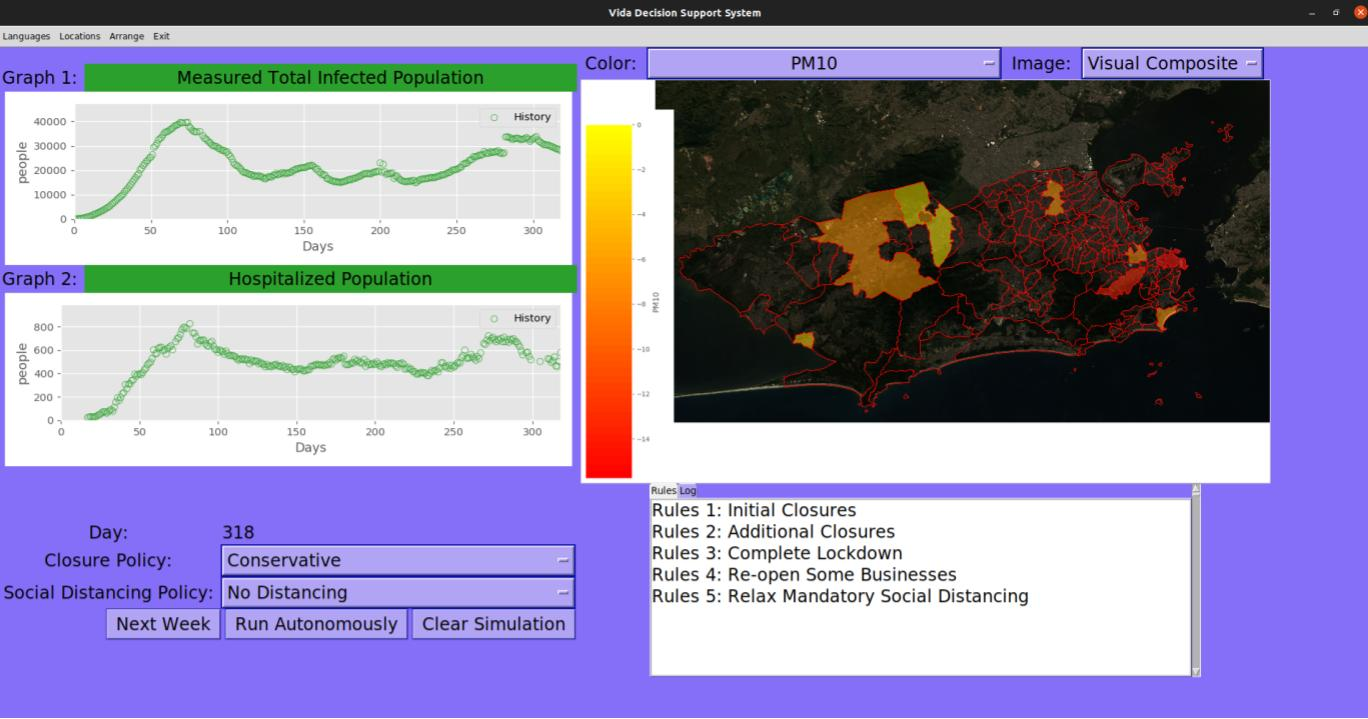
\includegraphics[width=0.85\textwidth]{Figures/chap5/VidaDesktopScreenshot.jpg}
\caption[Desktop Vida DSS Screenshot]{Screenshot of the desktop version of the Vida \ac{dss}. Currently showing the Rio de Janeiro study area.}
\label{fig:vidad}
\end{figure}


\subsection{Spatiotemporal Data Display}

This \ac{dss} can present temporal data, spatial data, and spatiotemporal data. The first of these is done through plots (visible on the left of Figure \ref{fig:vidad}), with the data visible in the plots controllable through dropdown menus. These are divided into eight categories:

\begin{itemize}[itemsep=0pt,parsep=0pt]
	\item{\textbf{Policies \& Actions:} Closure policies, social distancing policies, and curfews.}
	\item{\textbf{Health Parameters:} Various variables necessary for the \ac{sir} simulation but not directly measured, such as the typical contact rate between individuals or the average \ac{covid} illness duration.}
	\item{\textbf{Health Populations:} The various constitutive populations from which the \acl{sir} model is named. Includes both the recorded sizes of these populations and estimates of their actual size.}
	\item{\textbf{Health Flows:} Rates of change in the Health Populations.}
	\item{\textbf{Equipment Supplies:} Available supplies such as hospital beds and \ac{pcr} tests.}
	\item{\textbf{Environment:} Relevant environmental factors such as air quality.}
	\item{\textbf{Economic:} Metrics such as unemployment rates and \ac{gdp}.}
	\item{\textbf{Mobility:} Information pertaining to the movement of humans around the study areas.} 
\end{itemize}

Some of these datasets were based on direct collection and reporting by public health officials and other government agencies in each of the study areas. Others, such as the Hospitalization Rate, were calculated from the directed reported values (e.g. by taking the difference in hospitalized populations between each reporting period). Still others, such as the Hospitalization Likelihood, were set as constants with estimates based on the \ac{covid} literature and data from each particular study area. A full list of the temporal data available in these plots for each study area is available in Table \ref{tab:vida-temporal}.

The other two kinds of data are presented in the kinds of maps shown on the right in Figure \ref{fig:vidad}, which is currently displaying visual imagery of the Rio de Janeiro area overlaid with the most recent PM10 measurements from in-situ monitoring stations. Vector data is displayed using chloropleths, similarly to the \ac{dss} from Chapter \ref{ch:mangroves}. This typically included whatever of the temporal data was available in more geographically discrete forms, such as the various air quality measurements in Rio de Janeiro and Metropolitana.

The raster imagery, displayed underneath the semi-transparent chloropleths included a basic Landsat-based visual imagery composite, median urban nightlights, nightlights mean anomaly, and (in the Luanda case) Sentinel-5-based air quality measurements.

Should either the raster imagery or the vector geographic data be available at multiple points in time, additional slides appear at the bottom of the image to allow the user to select specific dates. Non-spatial data are saved in CSVs, vector spatial data in shapefiles, and raster spatial data in GeoTIFF format.

The arrangement of the plots and maps can be changed by the user with the Arrange drop-down menu in the top left. This allows for swapping their locations, displaying an additional two plots instead of the map, or displaying an additional map instead of the two plots.

\subsection{Scenario Generation}

In addition to presenting historical data, the desktop version of the \ac{dss} can also conduct public health simulations, using the system dynamics \ac{sir} model presented earlier. This simulations can either be run manually, with the user selecting specific policies at each week using the controls in the bottom left, or automatically for specified time periods, according to certain pre-coded decision rules (listed in the bottom right). These rules were based on the official policies of the location of interest. The user can then use the "Clear Simulation" button to reset the simulation in order to re-run the simulation with different inputs. Figure \ref{fig:vida-dss-simulation} shows a screenshot of the \ac{dss} once the simulation had been run in the pre-coded decision rule format for 300 days in the Rio de Janeiro study area. You can see it forecast an immediately forthcoming spike, followed by a major decrease in cases until, about 150 days later when another spike would occur.

\begin{figure}[!htb]
\centering
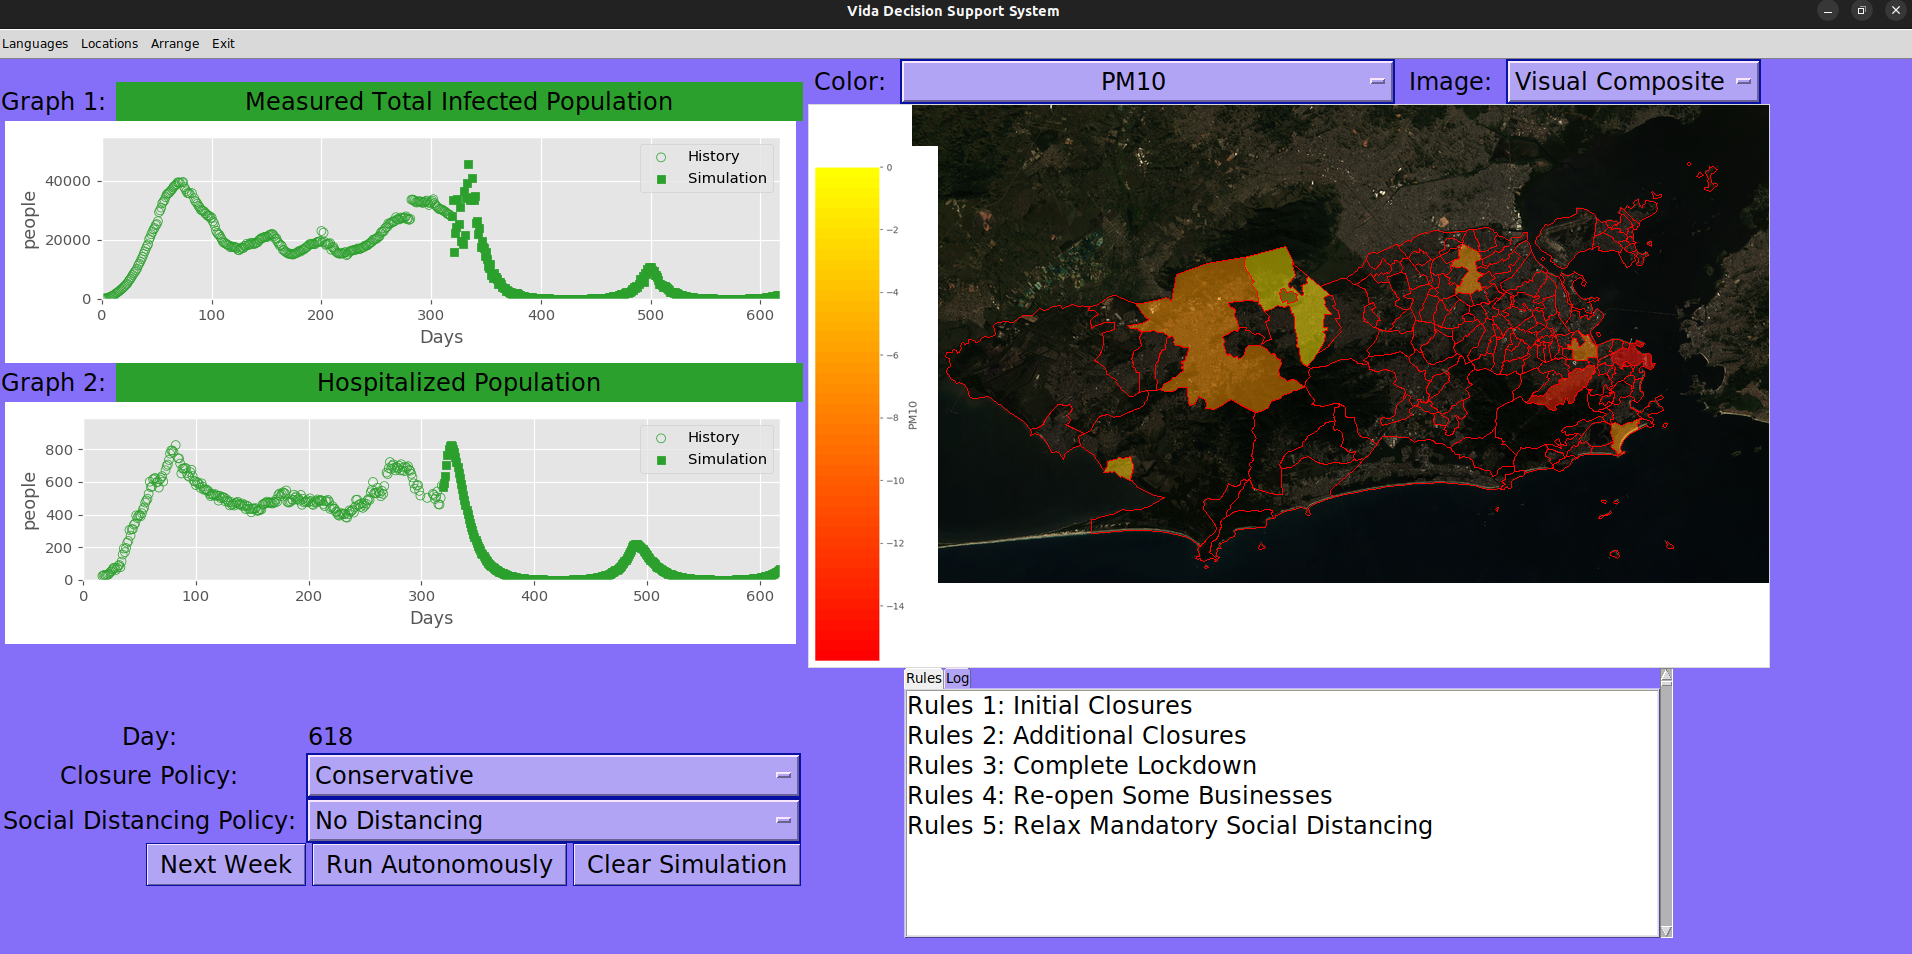
\includegraphics[width=0.85\textwidth]{Figures/chap5/vida-screenshot-simulation.png}
\caption[Vida DSS SIR Simulation Screenshot]{Screenshot of desktop Vida \ac{dss} once the \ac{sir} simulation had been run using the pre-coded decision rules for a period of 300 days in the Rio de Janeiro study area.}
\label{fig:vida-dss-simulation}
\end{figure}

Over the course of its development, the model was roughly calibrated using historical data, expanded as new dynamics become evident, and examined by public health experts. Various potential improvements are evident, including combining the \ac{sir} system dynamics model with an agent-based model to help address some of the deficiencies of the system dynamics approach \cite{ahmedVarianceSystemDynamics2012}, such as the lack of a spatial component.

\subsection{Experiment With An Online DSS}

In addition to the primary, desktop-based \ac{dss}, we experimented with the possibility of deploying an online \ac{dss}. This was done in collaboration with Blue Raster, who provided the software infrastructure and hosted it with their Esri's ArcGIS Online account. Ultimately this version of the Vida \ac{dss}, which was intended to be exploratory and as a proof-of-concept rather than the primary \ac{dss}, was only created for Boston \cite{bluerasterMITVidaSupportBoston2021} and Rio de Janeiro \cite{bluerasterRioJaneiroVida2021}, but not for the other study areas. 

This version, shown in Figure \ref{fig:vidab}, has different functionality than the desktop-based \ac{dss}. It focuses on the presentation of historical data (both temporal and spatial) and lacks simulation capability. It does however have the capability of showing more graphs at the same time, including allowing the user to merge multiple graphs into one for easy comparison, and an overall more streamlined interface. 

\begin{figure}[!htb]
\centering
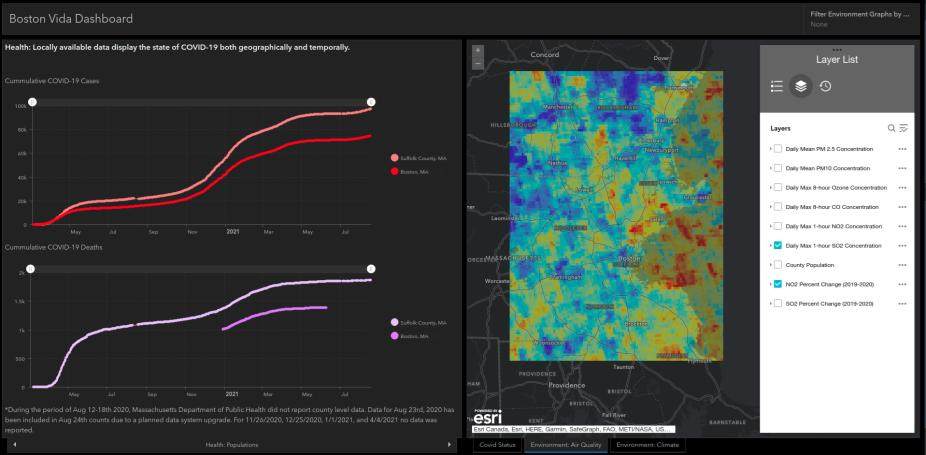
\includegraphics[width=0.85\textwidth]{Figures/chap5/VidaBlueScreenshot.jpg}
\caption{Prototype of the online version of the Vida user interface for Boston.}
\label{fig:vidab}
\end{figure}

\section{Collaborative Development Process} \label{sec:vida-collab}

The ways in which stakeholders were involved in setting priorities and requirements and surfacing data were detailed previously in Section \ref{sec:vida-saf}. These were by no means the extent of stakeholder collaboration as part of the Vida \ac{dss} International Network.

Various stakeholders participated in the development of the \ac{dss} itself. This took place in two primary ways. The first was actually working on the \ac{dss} itself either by directly submitting pull requests to the GitHub repository or by submitting proposed code changes to myself or Seamus Lombardo (who worked with me to manage the code base, as well as contributing significantly to the \ac{dss} code himself). The \ac{dss} code was structured to be quite modular, facilitating this process. In particular, stakeholders were able to add new historical datasets or components to the \ac{sir} model fairly readily, as well as improving or extending the display language translations. 

The second method was by providing feedback based on either presentations of the \acp{dss}, by accessing the online \ac{dss} themselves, or by running the desktop \ac{dss} themselves. The last of these was possible by either downloading and running the Python code or through the use of executable files that Lombardo and I put together using PyInstaller for specific stakeholders. These activities were conducted through weekly or biweekly meetings between the Boston-based research team and individual site representatives and through online collaboration via the local collaborators own online data repositories (e.g. Rio de Janeiro's Data.Rio \cite{institutopereirapassosDataRio2017} or Chile's Datos-\ac{covid} \cite{ministeriodecienciatecnologiaconocimientoeinnovacionDatosCOVID192021}), the Vida project's own code repository \cite{reidMITVidaRepository2021}, and through interaction with the browser-based version of the Vida \ac{dss} prototype \cite{bluerasterMITVidaSupportBoston2021}.

Beyond the \ac{dss} however, there was the additional objective to "shar[e] more general information and resources among the participants for responding to the pandemic." This was accomplished primarily accomplished through monthly, full Network meetings, at which participants presented and discussed useful lessons and tactics for addressing coronavirus response, including topics not directly related to Vida. Examples of such topics were how to implement wastewater viral testing and how to integrate the data generated into decision-making, how to approach health surveillance in elderly care facilities, and how to identify high vulnerability neighborhoods. An example agenda for can be seen in \ref{fig:vida-network-agenda}. These discussions, which cycled between several different times-of-day and days-of-week to maximize accessibility to participants from around the world, promoted innovation and enabled cross-location learning that may not otherwise occur. They also enabled participants to communicate with one another in a shared, non-English language when this was helpful. Specific examples of such benefits include:

\begin{itemize}[itemsep=0pt,parsep=0pt]
	\item{Presentations on how Rio de Janeiro and Chile were making \ac{covid} case data and other data available online prompted Indonesia stakeholders to similarly publish data online using ArcGIS Online \cite{indonesiaministryofhealthDataHarianKasus2023}.}
	\item{A presentation by Paulina Assmann on setting up a wastewater surveillance system for \ac{covid} led to discussion and followup meetings with participants about setting up similar systems in Mexico and Brazil \cite{assmannBuildingWastewaterSurveillance2021}. Ultimately such systems were set up in both of those locations, though I cannot claim with any surety that this interaction was directly responsible.}
	\item{Future, post-pandemic projects and collaborations were inspired, including a flood resilience \ac{evdt} project in Pekalongan, Indonesia and using \ac{eo} imagery to identify socioeconomically vulnerable areas of Mexico.}
\end{itemize}

Recordings of these full Network meetings were made available online, along with slides from presentations.

We also proposed organizing dedicated webinars on various topics, hosted by relevant experts from among the participants, but surveys of Network participants suggested that this was not a priority, so this was not pursued. 

\begin{figure}[!htb]
\centering

\includegraphics[width=0.5\textwidth]{Figures/chap5/vida-network-agenda.png}
\caption{Vida Network Meeting Agenda}
\label{fig:vida-network-agenda}
\end{figure}

\section{Discussion} \label{sec:vida-discuss}

This section will discuss the results and lessons of the previous sections of this chapter. It starts by considering the various limitations of this work and the potential for future work, before discussing the lessons this project have for the \ac{evdt} Framework in general.

\subsection{Methodological Limitations \& Potential Improvements}

The combination of the novelty of the \ac{covid} pandemic (limiting prior understanding of its potential impacts), the suddenness of its onset (with the resulting limitations in available data), the juggling of the priorities for multiple different study areas, and the limitations of my own abilities and those of the US Vida team meant that there were various shortcomings in this project's implementation. There are also a variety of potential future opportunities, both \ac{evdt} and otherwise, in this space. This section considers both.

\subsubsection{Environment}

The air quality analysis presented here was based on a relatively small number of in-situ monitoring stations throughout Rio de Janeiro and the Metropolitana region. This limited our ability to connect these changes with \ac{covid} cases, nightlights, or other subjects of analysis that had much greater spatial detail. As mentioned in Section \ref{sec:vida-evdt-e-method}, some visualizations of SO2 and NO2 did make their way into the desktop \ac{dss} for the Luanda area, this was not repeated for the study areas with in-situ stations. Connecting the two could allow for calibrating the \ac{eo}-based air quality data and a better understanding of spatial variation across each of the study areas.

\subsubsection{Public Health}

The \ac{sir} public health model used in this project is relatively simple. This had certain benefits, including allowing for fast simulations within the \ac{dss}. It obviously comes with various limitations. Perhaps chief among these was the lack of spatial differentiation within each study area (except for Indonesia, in which separate models were run for Java and Sulawesi). Such bulk simulations have some utility for a municipality like Rio de Janeiro, as most \ac{covid} response policies applied equally across the city. It makes less sense for a larger region like Metropolitana or Java, which is likely to have different dynamics at play in different parts of the region and have policies being made for particular municipalities or sub-regions.

It may make sense to extent the concept that was used for Java and Sulawesi, to run distinct \ac{sir} models in parallel at the scale of primary policymaking while also adding in connections between these subregions based on human travel and infection vectors.

Another potential improvement is to add a stochastic element to the \ac{sir} model. Many of the underlying parameters, such as the likelihood of infection upon contact and the number of unreported \ac{covid} cases, were not directly measured and were instead estimates based on the best available evidence. These estimates have some (sometimes large) level of uncertainty. An improved model could integrate these uncertainty levels and run in a Monte Carlo fashion, presenting a distribution of possible future scenarios rather than a single one.

Both simulations would come at the cost of additional required computation power, but the speed of the current version of the \ac{dss} suggests that significant additional computational complexity could be accommodated without drastically impacting usability.

\subsubsection{Vulnerability}

The relatively poor temporal and spatial resolution of many economic metrics (unemployment rates, GDP, etc.) limited our ability to make serious connections between \ac{covid} and socioeconomic impacts during this project. One potential solution to this is to collect the missing data to whatever extent is feasible. This was the intent of the Invisible Variables Initiative, which conducted longitudinal, qualitative surveys of individuals over the course of the pandemic to better understand impacts of \ac{covid} on individuals safety, means, and autonomy \cite{turnerInvisibleVariablesImpact2021}. This initiative had a relatively small sample size and was only conducted for the Greater Boston area, but the concept could be extended to other areas and the resulting findings could help inform future disease-response \ac{evdt} projects.

Our mobility analysis was limited by the lack of publicly available pre-covid data. Both the Google \ac{covid} Community Mobility Reports \cite{googleCOVID19CommunityMobility} and the Chilean Indice de Movilidad \cite{ministeriodecienciatecnologiaconocimientoeinnovacionDatosCOVID192021} only reported data for mid-to-late February 2020 onward. This prevented us from correcting for any periodic or secular trends in the data unrelated to \ac{covid} (as was done for the air quality analysis). Both also stopped being updated in 2022, meaning that such corrections will not be possible even for future pandemics. 

One possibility to help address this, as well as to add a higher level of spatial resolution to such mobility data (which is typically at the city, county, or provincial level) is to connect it with urban nightlight data or some other potential \ac{eo}-based proxy. Nightlight data has a history of use as a proxy for economic activity \cite{delvalleMangrovesProtectCoastal2020}. Some post-pandemic studies have found correlations with regional mobility data (such as the Google \ac{covid} Community Mobility Reports) and urban nightlight data \cite{schweikertMobilityNightlightsAir2022}. If researchers could access more spatially fine-grain telecoms-based mobility data, such as what the City Science Research Group had for the microstate of Andorra \cite{doorleyMobilityCOVID19Andorra2022}, these correlations might be able to be extended to the scale of neighborhoods. Alternatively, so-called "synthetic population models" could be used in lieu of actual mobility data \cite{akbarpourSocioeconomicNetworkHeterogeneity2020}.

\subsubsection{Decision-Making}

As was discussed in Section \ref{sec:vida-evdt-decision-method}, we never completed the second, more systematic quantitative categorization of \ac{covid} response policies for the study areas. If we had, the next step would have been to develop either a composite score or individual policy type scores to provide the Public Health model. These connections would be based on the current understanding of the impact (public health and otherwise) that various policies have. This is an area with a rapidly increasing corpus in the literature (e.g. \cite{bennettAllThingsEqual2021, wibbensWhichCOVIDPolicies2020, dergiadesEffectivenessGovernmentPolicies2020}). As this corpus develops, care must be taken to identify what was unique to the \ac{covid} pandemic and what is generalizable to future outbreaks.

\subsubsection{Technology}

As with the case study presented in Chapter \ref{ch:mangroves}, the Technology component was the most underdeveloped in this project. It primarily came into play with some minor use of information about testing regimes in each study area to estimate the number of unreported \ac{covid} cases. One potential improvement would be to include the selection of a testing regime as a policy choice in the \ac{dss}. This would require more detailed knowledge that was available to us regarding the influence of testing regimes on \ac{covid} cases or other phenomena, but this might be remedied by an increasing body of literature on the subject \cite{cordesSpatialAnalysisCOVID192020, souchCommentaryRuralUrban2021}.

\subsubsection{Stakeholder Collaboration and Engagement}

Compared to the \ref{ch:mangroves} case study, the Vida project had a higher level of stakeholder participation and collaboration in the development of the \ac{dss} and in conducting the \ac{evdt} analyses, with some of the stakeholders contributing relevant analyses of their own as well. This is likely partially attributable to the urgency of the pandemic and to the fact that the pandemic forced many of us to become more comfortable with remote collaboration. 

This project did suffer from not significantly engaging a diverse set of stakeholders within each study area however. Pressured by the urgency of the pandemic and the complications inherent to handling so many different study areas simultaneously, we rushed through much of the stakeholder analysis portion of the \ac{saf}. While many stakeholders beyond the primary contacts listed in Table \ref{tab:vida_participants} were briefly involved in discussions, meetings, and presentations, few were engaged in any sustained manner. This represents a major area for improvement, as is discussed further in Section \ref{sec:vida-lessons}.

One of the more successful forms of stakeholder collaboration and engagement were the multilateral Vida Network meetings. These resulted in the continuation of such meetings for a more general \ac{evdt} community audience after the conclusion of the Vida project.

\subsubsection{Decision-Support System}

The \acp{dss} developed in these projects were not final products and had numerous potential avenues for improvement. These included:

\begin{enumerate}[itemsep=0pt,parsep=0pt]
    \item Automating data updates and ingestion, allowing the \ac{dss} to remain up to date without manual intervention from the US team or others. 
    \item Standardizing architecture and implementation to facilitate reuse of model components. This was already partially done, as much of the desktop \ac{dss} code was based on code from the Chapter \ref{ch:mangroves} \ac{dss}, but further improvements are certainly possible.
    \item Add simulation capabilities to the online version
    \item Improving visualizations, including adding the ability to zoom in/out on the maps.
    \item Adding a spatial component to the epidemiological model, as was discussed above.
    \item Continue air quality, nightlight, and mobility analysis with the potential for integrating these more fully into the simulation capability. 
\end{enumerate}

That said, the goal of this project was not for the Space Enabled team to indefinitely improve and maintain these \acp{dss}. Instead we were seeking to provide what decision support we could, while providing a proof-of-concept and some level of capacity building for the collaborating study areas. 

\subsection{Lessons Learned for the EVDT Framework} \label{sec:vida-lessons}

As discussed at the beginning of this chapter, this case study diverged significantly from the original concept of an \ac{evdt} project both in its speed and in its inclusion of some many distinct study areas. This resulted in numerous methodological deviations. As such, it cannot be considered to be a demonstration or test of the \ac{evdt} Framework proper. Nonetheless, it is important to understand how approaches breakdown or stand strong during disasters, so the following lessons were drawn with this in mind.

\textbf{The benefits of multi-study-area or multi-project communication and collaboration.} As mentioned earlier, the Vida International Network has facilitated international collaboration, allowing participants to share innovations and insights from their \ac{covid} response efforts. It has also encouraged intra-country collaboration by providing a motivation for outreach between government officials, academic researchers, and community leaders in order to fill data gaps and answer pressing questions. This process has also raised awareness of the utility of space-based \ac{eo} data, potentially preparing participants for future pandemic and non-pandemic applications. 

The success of the multilateral Network meetings prompted us to continue such meetings for a more general EVDT community audience, as well as to consider other potential means of engagement such as webinars or online resources. This likely would not have occurred if we had continued to pursue more individual, siloed \ac{evdt} projects as was the norm.

\textbf{The importance of clearly scoped situation and use that can be completed within team resources, particularly during an emergency situation.} Overall, the Vida project included many unsuccessful experiments (such as monitoring vehicle traffic) and disconnected components (such as the separate in-situ and \ac{eo}-based air quality analyses). We generated some interesting results that did not find their way into the \ac{dss} proper or to supporting decision-making in other ways. This was very unlike the Chapter \ref{ch:mangroves} case study that had a clear through-line to the analyses and the \ac{dss} (see Figure \ref{fig:evdt-dss-flow}). This was partially due to the rushed stakeholder analysis, which was in turn due to the urgency of the situation and the complexity of multiple study areas. As such, it was potentially unavoidable in this case study but nonetheless represents a cautionary tale for future \ac{evdt} analyses.

It was also partially due to the how thin the Space Enabled team was spread by this project. I was the only one with experience with a prior \ac{evdt} project directly involved with Vida. Seamus Lombardo, who was an invaluable asset here, had only recently joined the lab and had significant on-the-job learning ahead of him. We both ended up being the primary point of contact for multiple regions (I primarily took on the Latin American study areas, Lombardo primarily took on Indonesia and Angola, but this was subject to significant flux over the course of the project). This limited our ability to do deep dives into any particular study area and tailor the \ac{dss} to the needs of particular study areas or stakeholders.

In the face of such pressure, we tended to default to responding most quickly to clearly articulated requests that were immediately actionable. \ac{ggpen} was interested in shipping traffic off the coast of Luanda and in outdoor fires across the country, so we provided that. The Universitas Diponegoro in Indonesia requested a bifurcated epidemiological model for the geographically separate islands of Java and Sulawesi. Various stakeholders had different datasets that they wished included (\ac{ipp} and air quality, \ac{minciencia} and mobility, etc.). Serving the clearly stated desires of these particular stakeholders is all well and good, but it did distract us from properly engaging with a diverse set of stakeholders in each study area, as was done more fully in Chapter \ref{ch:mangroves}. Did the public in Luanda need information on ship traffic? Did other government agencies outside of \ac{ggpen}? What other analysis could we have been prioritizing? We do not know and this should concern us.

The lesson here bolsters the \ac{evdt} Framework's methodological focus on a particular study area for a given project (while still encouraging re-use across projects). 

\textbf{The power of reusing assets and building upon experience, particularly when a rapid response effort is required.} While the previous lesson focuses on the limitations of this case study, I also wish to note that this project was able to deliver concrete results to stakeholders on an accelerated timeline, in a disruptive environment, and for several different study areas. This was an ambitious undertaking that would not have been possible without the various forms of expertise that the Local Context Area Experts and Technical Area Experts had. It also would not have been possible if this had been the first \ac{evdt} project. Reusing code from the Chapter \ref{ch:mangroves} \ac{dss} and workflows for analyzing \ac{eo} data were invaluable, as was a higher level of familiarity with the \ac{evdt} Framework that I and other participants had as a result of previous projects.


\section{Conclusion} \label{sec:vida-concl}

This chapter presented one of the more unique implementations of the \ac{evdt} framework. Where most other \ac{evdt} applications to date have focused on a particular study area and little urgency (at least on the scale of weeks to months), this project sought to rapidly support \ac{covid} response across several different regions around the world. To this end, I detailed the situation that these regions (and the world at large) faced and what the stakeholder needs were. This was followed by a series of analyses on how air quality, nightlights, \ac{covid} cases, mobility, and policies. These were used to construct two prototype \acp{dss} for viewing \ac{covid}-related data and simulating various policy outcomes.

In doing so, this case study not only supported stakeholders' decision-making, but it also provided a demonstrated of the \ac{evdt} Framework, thereby helping to respond to Research Question 2: "Does the \ac{evdt} Framework effectively support decision-making in in complex \ac{sets}?"

This implementation was not without its flaws and this experience informed refinements of the \ac{evdt} Framework. The following chapter will use these lessons to evaluate the framework itself.

